\begin{abstract}
In the initial phase of \sw (SW1), volunteers were invited to search the CFHTLS sky survey to look for gravitational lenses.
Here we report on a web application that gives experienced volunteers the opportunity to model the candidates that have been identified.
In order to gauge the quality of the models that were being rendered, these same volunteers were invited to model a sample of 29 simulated lenses.
The models were then examined in greater detail, with particular attention being paid to the following:
(i)~identification of image parities and time arrivals;
(ii)~the mean convergence (equivalent to the enclosed mass), and finally;
(iii)~the performance of a volunteer vs. a professional.
In most cases, the volunteers were found to correctly identify the image parities and time arrivals.
% Einstein radius +~20%
 along with a mean convergence that was well constrained within the image region;
In all, the results could be comparable to that of a professional.
\end{abstract}

\begin{keywords}
\end{keywords}

\section{Introduction}


Galaxies and clusters of galaxies are considered to be the largest structures in the known Universe. When one questions their formation,  the present picture suggests that gravitational instabilities  (observable as fluctuations of the microwave background) %TODO \todo[red]{not too sure of the relevance of this statement} 
 - caused a collapse into gravitationally bound structures. %TODO\todo[yellow]{clarification needed: are they becoming gravitationally bound structures, or are they collapsing into objects that are already gravitationally bound? I know it is most probably the later, but it is a bit ambiguous}   
The initial collapse would have been dominated by dark matter, but once deep wells had appeared in the gravitational potential, gas would have started falling into those wells. 
%TODO \todo[red]{not too sure of this wording}
Through atomic processes,
%TODO \todo[yellow]{perhaps we need to clarify those processes or are they generally know?}
 the gravitational potential energy of this gas would of been radiated away, leading to the formation of the largest stars. 
%TODO \todo[red]{or perhaps just stars?}
In turn, galaxies and clusters of galaxies would form, all the time merging and changing their form.
This rough outline is now well established, but in order to satisfy our understanding of this process, there are many puzzles  that remain to be solved. For progress to be made, we need to extend our knowledge of dark matter. Gravitational lensing has proven as a particularly attractive way of studying dark matter as it is only dependant on mass.
%TODO \todo[yellow]{silly question, but shouldn't we briefly explain why it is only dependant on mass? or should everyone already reading this paper know that? or is it explained later?}


There are many manifestations of gravitational lensing in astrophysics,
but the most spectacular are multiple images.  Gravitational lensing
depends on the sky-projection mass density, and this fact has a
counter-intuitive consequence: nearby galaxies do not produce multiple
images, because their projected density is not high enough, but beyond
100~Mpc or so, most galaxies are potential lenses.  Even so, for a
potential lens to really act as a lens, a background source in the close-by
region is required.  So, in practice galaxies are very rarely observed
as lens.  The same tendency applies to clusters of galaxies, but since
clusters are bigger, they are more likely lens-like.

In lensing galaxies, the observable features usually involve a single
object multiply imaged.  It is therefore desirable to have large
numbers of lenses, and this is the strategy researchers are following.  The
largest single study so far uses 58 lenses \citep{2009ApJ...703L..51K}.
Other studies have compared lens models in more detail with stellar
mass \citep{2011ApJ...740...97L} or used time-delay information from
lensed quasars to infer the Hubble time
\citep{2008ApJ...679...17C,2010ApJ...712.1378P}.

The trend is clear: researchers want to find many more lenses and
model them in more sophisticated ways.

\begin{figure}
\centering
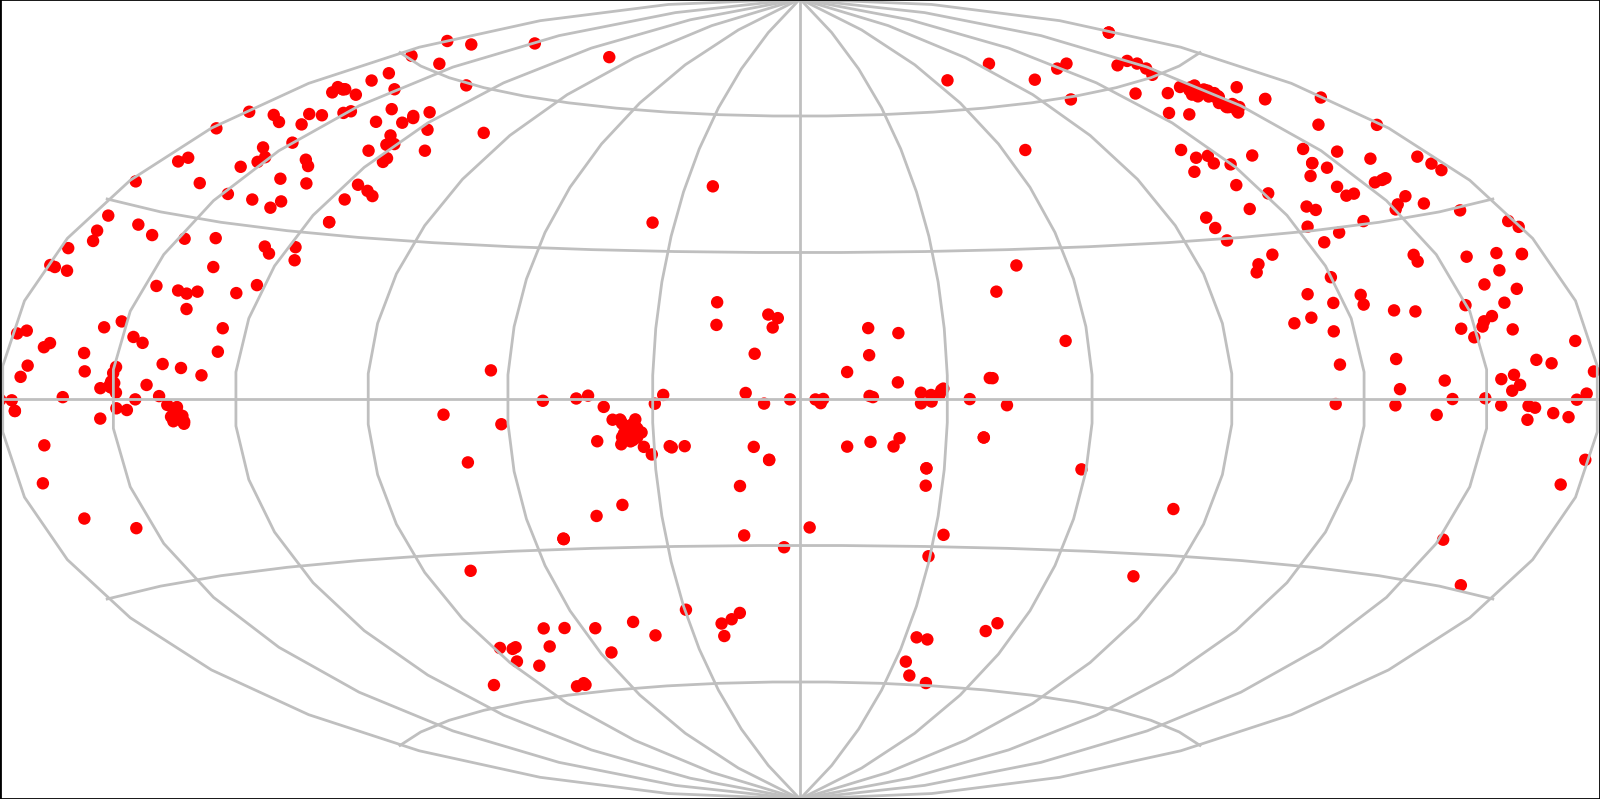
\includegraphics[width=0.9\hsize]{fig/lenssky}
\caption{Sky distribution of 423 published lenses considered secure as
  of January 2014 (from the Masterlens catalog at the University of
  Utah, maintained by Joel Brownstein and Leonidas Moustakas.) The map
  is in Hammer-Aitoff projection, with North up and $\rm RA=0$ in the
  middle.  The empty swathes to the left and right of center are the
  Milky Way.}
\label{fig:masterlens}
\end{figure}

A good summary of the observational situation is offered by
Figure~\ref{fig:masterlens}, which shows known secure multiply-imaging
lenses.  The non-uniformity on the sky is not intrinsic, it just
indicates the density of deep surveys up to 2013.  At HST resolution,
of order 1~square degree of sky must be searched to find a lens.
Older ground-based surveys yield a lens per roughly 10~square degree
of survey area.  By the large surveys starting now
(DES\footnote{\tt http://pan-starrs.ifa.hawaii.edu} or
PanStarrs\footnote{\tt http://www.darkenergysurvey.org}) the expected
yield is something in between.  Given their unprecedented survey area,
these are likely to yield thousands of lenses.  Over the 2020s,
LSST\footnote{\tt http://www.lsst.org/} can be expected to give us ten
thousand lenses.

The question now arises: can lenses be found and modeled
automatically in large surveys?  Work using software robots
\citep{2009ApJ...694..924M} gives some interesting and unexpected
results.  In clean lensing system in uncrowded fields with high
signal-to-noise, the robots do very well.  In most situations,
however, robots miss lenses (low completeness) or contaminate the
results with non-lenses (low purity).  Robots can be made to
prioritize completeness or purity, but they cannot deliver both.

In response to the lessons learned from automated lens searches, the
{\em Spacewarps\/} project\footnote{\tt http://www.spacewarps.org}
 has been launched.  {\em Spacewarps\/} is
part of the {\em Zooniverse\/} family of citizen-science
projects,\footnote{\tt http://www.zooniverse.org} where members of the
public are invited to analyze different kinds of scientific data which
are too difficult for robots and too large for specialists.  In {\em
 Spacewarps\/} itself, survey sky images are presented for volunteers to identify lens candidates.  The first tranche of survey data, introduced from May 2013, is an area of $\sim172$ square
degrees (or a quarter of a percent of the sky) from the Canada-France-Hawaii Telescope Legacy Survey.
 The survey is divided into patches of $440\times 440$ pixels, each of
which is seen by ten volunteers.  Simulated lenses are mixed in with
the data, both to help train volunteers on what to look for, and to
estimate completeness and purity.
These data had previously been analyzed by robots \cite{Gavazzi2012, More2012ApJ}.  
  A list of candidates is being
processed, but intermediate results show some very good candidates, as
well as re-discoveries of candidates previously found robotically.

These encouraging results now raise the question: could modeling of
the lenses also be done by volunteers?  Modeling is a much more
difficult task than searching for lens candidates, as it requires some
expert knowledge.  Nonetheless, a panel of the {\em Spacewarps\/}
volunteers is quite experienced from earlier projects, having spent a
thousand hours or more with data.  Some of these experienced
volunteers are very interested in more demanding projects.  This also
is a general trend \citep[cf.][]{Khatib22112011}.  The present project
then suggests itself.

The purpose of this study was to provide a means to model a large number of gravitational lenses by showing that gravitational lens modeling can be learned / done by volunteers.
We suggest, that volunteers will be as successful as professionals with modeling if provided with an easy to use tool with visual feedback (What you see is what you get, WYSIWYG) and a minimal set of instructions.
Volunteers will then crowd work (using buzz word here ;) ) / work collaborative on modeling lenses from several sources / groups at a central place.
Since this is an iterative learning process, the more involved volunteers will quickly gain knowledge that can be passed down to new volunteers.
That creates a social structure that scales well with the number of volunteers, as other projects have already shown. %TODO \needcite
Finding people working as volunteers has been shown to be successful last but not least by \sw and the whole galaxy zoo project.
To test the people's abilities, we investigated the performance of a few volunteers modeling a set of simulated lenses.
We tested the ability to correctly identify lensed images and reproduce similar mass map of the lens.


\section{A lens modeling program}

It is well known that making a scientific contribution is a central
motivation cited by citizen-science volunteers.  So for a lens
modeler in a citizen-science project, nobody wants that it should
sacrifice scientific usefulness in order to be fun to use.  That said,
being aesthetically pleasing and having a short initial learning curve
are also essential qualities.  Also desirable is that the user is
encouraged/challenged to go deeper and wider into the subject.
Yet another aspect is enabling small incremental contributions
by different people.  \spl tries to address all of these.

\subsection{Fermat's Principle and ``spaghetti'' contours} \label{sec:Fermat}

There are several ways to understand the formation of arcs and
multiple images in gravitational lensing.  We will follow some ideas
originally introduced by \cite{1986ApJ...310..568B}, based on Fermat's
principle.  The key to this approach is an abstract construct called
the {\em arrival-time surface.}  This surface cannot itself be
observed, but several observable quantities can be derived from it.

\begin{equation} \label{eq:tgeom}
\tgeom(x,y) \propto (x-x_s)^2 + (y-s_y)^2 \,.
\end{equation}

The gravitational time delay can be expressed in an implicit form: the
value of $\tgrav$ through $(x,y)$ equals its average value on the
circumference of a small circle centred at $(x,y)$, plus a constant
times the mass within that circle.  The proportionality constant is
$2G/c^3$ times the cosmological expansion factor $(1+z_L)$. Thus
\begin{equation} \label{eq:tgrav}
\tgrav(x,y) = \left\langle \tgrav(x_\subcirc,y_\subcirc) \right\rangle
              + (1+z_L) \frac{2G}{c^3} M(x_\subbullet,y_\subbullet) \,.
\end{equation}
We have used $(x_\subcirc,y_\subcirc)$ to denote the circumference of
a circle, and $(x_\subbullet,y_\subbullet)$ to indicate the integrated
mass within the circle.

\begin{equation} \label{eq:kappa}
\kappa(x,y) \propto \Sigma(x,y) \,.
\end{equation}

Incidentally, $\kappa$ has a second meaning, as well as
being a dimensionless form of the projected density: it also
measures how a bundle of light rays is brought together by
gravitational lensing, and is called the {\em convergence}.

Consider a gravitational lens.  As in most astrophysical lensing, this
lens is `thin' along the line of sight, and effectively lies on a
plane.  Let $x,y$ be coordinates on this plane.  These coordinates
measure ordinary physical lengths (meters, etc) on the lens plane.
Let there be a point source of light at $x=0,y=0$ but far behind the
lens plane.  Now imagine a light ray coming from the source to the
lens plane $(x,y)$ and then changing its path to reach the observer.
The observer would see the source apparently behind $(x,y)$ the
lens.  If this happened, the light ray would have taken a longer path
than having come directly to the observer.  The geometrical path
difference would be $\propto x^2 + y^2$ for small angles.  Let us
define
\begin{equation} \label{eq:Ageom}
A_{\rm geom}(x,y) = \half(x^2 + y^2) \,.
\end{equation}
As written, this looks an area.  But we can also think of it as a
time delay introduced by the light ray bending --- with an unwritten
constant factor.  That factor is basically the lens distance divided by the
speed of light; the precise expression has to take the expansion of
the Universe into account, and is given in the Appendix.  The top part
of \figref{arriv} shows what $A_{\rm geom}$ looks like: it is
just a paraboloid.  The minimum of the surface is at the source, and
that is where, according to Fermat's principle, the image will be.
The rest of the arrival-time surface is just an imaginary surface.

\begin{figure}
\centering
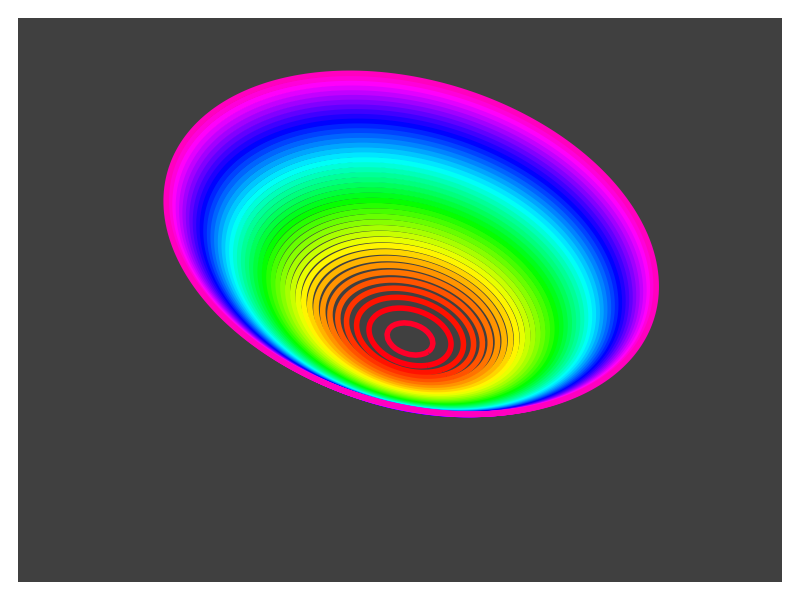
\includegraphics[width=\columnwidth]{fig/arriv_0}
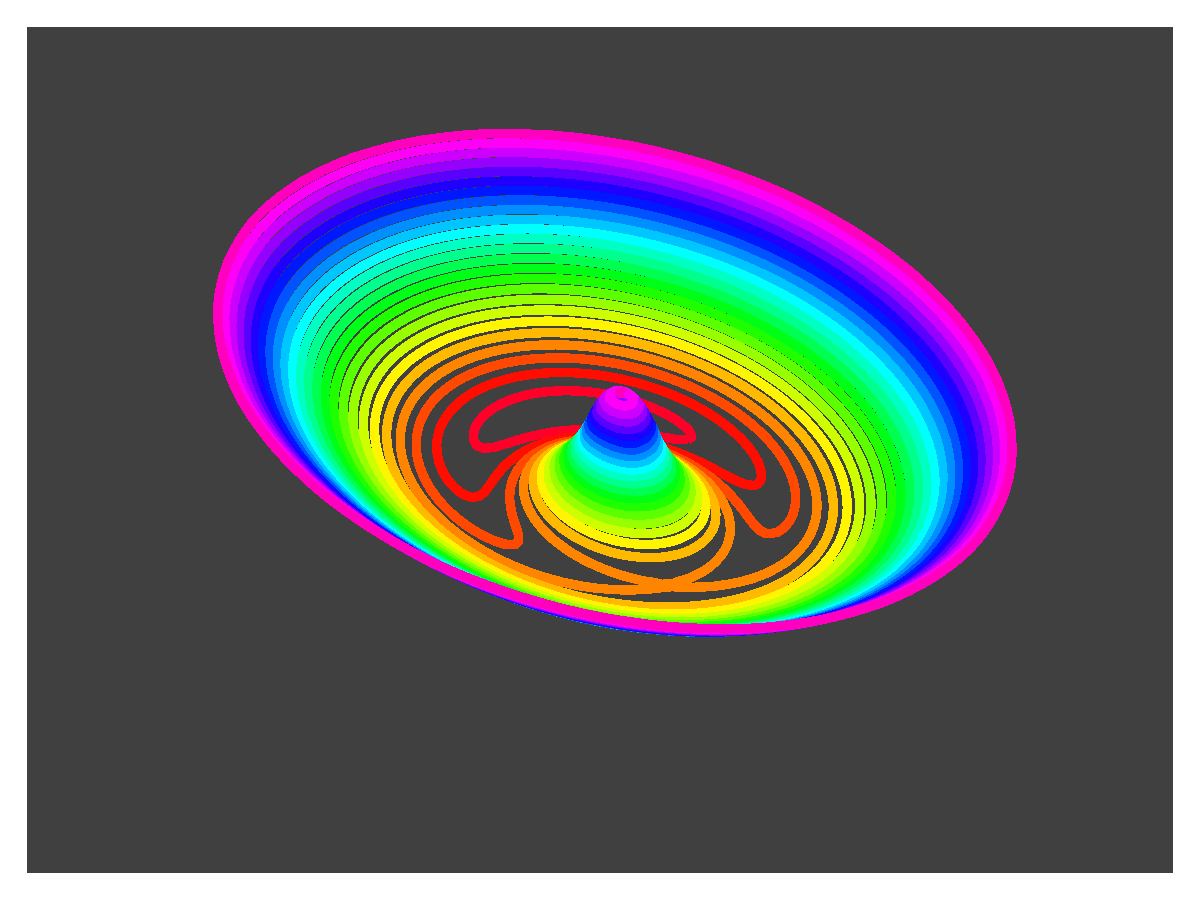
\includegraphics[width=\columnwidth]{fig/arriv_1}
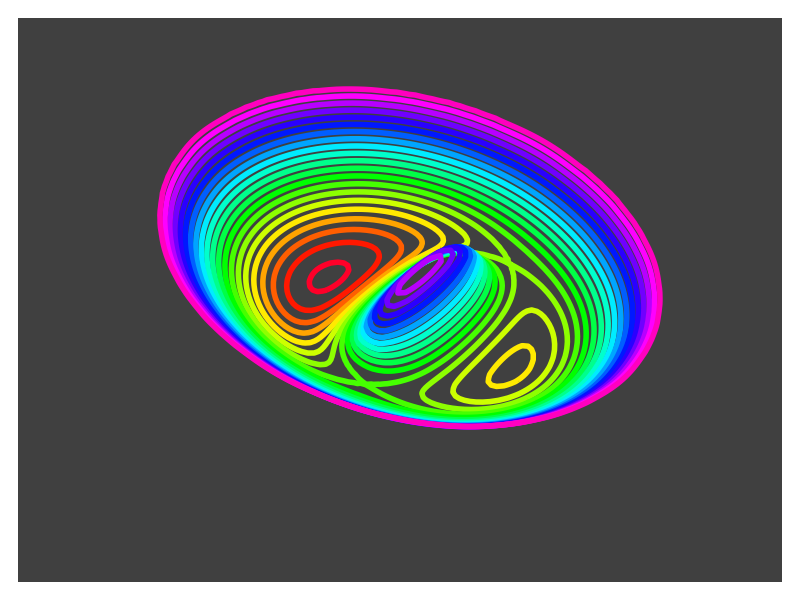
\includegraphics[width=\columnwidth]{fig/arriv_2}
\caption{Perspective views and contour maps of example arrival time
  surfaces.  Contours are coloured in rainbow order (red: least delay,
  violet: highest delay).  {\em Upper panel:\/} No lens, hence showing
  the parabolic shape of the geometrical time delay.  The image would
  be at the bottom, coinciding with the source. {\em Middle panel:\/}
  A circular lensing mass (offset from the source) has been added,
  which has pushed the minimum to one side and introduced a maximum
  and saddle point, each corresponding to an image.  The saddle-point
  is characterized by a self-crossing ``spaghetti'' contour. {\em
    Lower panel:\/} An elongated lensing mass has been added.  There
  are now two minima, two saddle points, and a maximum, each
  corresponding to an image.  Note the two self-crossing spaghetti
  contours associated with the saddle points.}
\label{fig:arriv}
\end{figure}

The geometrical time delay \eqref{eq:Ageom} is not the only one.  The
warping of space by a gravitational field introduces a further time
delay $A_{\rm grav}$.  The arrival time of the light ray, compared to
what it would have been with no lensing, is
\begin{equation} \label{eq:Aarriv}
\hbox{arrival time} = t_{\rm geom} + t_{\rm grav} \,.
\end{equation}
We can also express $A_{\rm grav}$ as an area, with the same implicit
constant factor that makes it a time.  The expression, however, is
more complicated.  We first introduce the notation $\nabla^2 f(x,y)$
to denote
\begin{equation}
 \frac{ f(x+\Delta x, y) + f(x-\Delta x, y) +
        f(x, y+\Delta y) + f(x, y-\Delta y) - 4 f(x,y) }
      {\Delta x \; \Delta y}
\end{equation}
in the limit of $\Delta x,\Delta y$ small.  Then we write the
projected mass density of the lens, which would be in $\rm
kg\,m^{-2}$, in special units (given in the Appendix) such that the
surface density becomes a dimensionless field $\kappa(x,y)$.  Then
\begin{equation} \label{eq:Poisson}
\nabla^2 A_{\rm grav}(x,y) = -2\kappa(x,y) \,.
\end{equation}
Note that $A_{\rm grav}(x,y)$ is not given explicitly in terms of
$\kappa(x,y)$, but as a differential equation that must be solved.
Equations of the type \eqref{eq:Poisson} are, however, well known (as
Poisson's equation in two dimensions), and there are techniques for
solving them.  

What is the effect of mass on the arrival-time surface?  If the mass
distribution $\kappa(x,y)$ is circular, $A_{\rm grav}(x,y)$ will have
a peak at the center of that circle.  But if the mass is not precisely
in front of the source, the arrival-time surface will not be circular
any more.  The result is illustrated in the middle part of
\figref{arriv}.  In addition to the maximum, there is now a
minimum and a saddle point.  According to Fermat's principle, images
appear at maximum and saddle points as well as minimum.  If the mass
distribution is non-circular, more images can appear.  The lower
example in \figref{arriv} shows the arrival-time surface due
to an elongated mass.  There is still a maximum, part of an elongated
hill, and around it there are two minima and two saddle points.

So far we have considered a single point source.  What if there is an
extended source?  To understand this, let us consider what happens if
we move the original point source slightly, or equivalently, keep the
original point source behind $x=0,y=0$ and move the lens slightly.
The contours of constant arrival time will naturally move slightly,
and so will the images.  The movement of the contours will be most
noticeable where the contours are far apart, that is where the
arrival-time surface is nearly flat.  As is evident from
\figref{arriv}, this is the region where the minimum and saddle
points lie, or near the images.  In this region, points on the source
that are close together produce images that are comparatively far
apart.  In other words, the image is highly magnified.  In summary,
lower curvature in the arrival-time surface for a point source implies
larger magnification of an extended source.  Conversely, where the
arrival-time surface is strongly curved, the image will be
demagnified.  We see from \figref{arriv} that the arrival-time
surface tends to be highly curved near the maximum.  Hence maximum tend
to be demagnified.  In practice, maxima of the arrival time are nearly
always too faint to see. The minima and saddle points dominate.

In the lensed examples in \figref{arriv}, the maximum in each
case is evident, but how can we distinguish the minima from the saddle
points?  The key is to examine the contours of equal arrival time.
Contour curves loop around a minimum or a maximum, but near a saddle
point, the contours do not loop around, instead they approach and then
pull away.  The contour curve precisely level with a saddle point
forms an X at the saddle point.  In \figref{arriv}, one such X
is evident.  In other cases the X contour passing through the saddle
point is not itself plotted, but we can tell by the other contours where
the X would be.  These self-crossing contours will play a special role
in the following.

\FloatBarrier
\subsection{\spl} \label{sec:SpaghettiLens}

\spl implements the ideas of the arrival-time surface into a modeling
program.

The first modeling step with \spl is for the user to call up the \sw
of interest, and make an educated guess for the topography of the
arrival-time surface --- specifically, the locations of the maxima,
minima and saddle points that correspond to images of the brightest
part of the source.  Input is given by tracing a proposal for the
saddle-point contours.  \Figref{input-spag} shows some example
inputs --- and incidentally also indicates the origin of the name
\spl.

\spl, as implemented so far, assumes that the lens is dominated by a
single galaxy, and that the center of that galaxy is the sole maximum.
Once the maximum has been identified, we wish to characterize the rest
of the arrival-time surface in relation to it.  From geometry, any
surface that has a central maximum and goes high at the edges must
have a lima\c con-like contour, meaning a two-looped curve with one
loop inside the other.  The maximum lies within the inner loop, a
minimum lies between the two loops, and a saddle point lies at the
self-intersection of the contour.  The top panel of
\figref{input-spag} shows an example: red marks a suggested
maximum, green a saddle point, and blue a minimum.  (The small pink
dots are just help sketch the proposed contour.)  The middle and lower
panels of \figref{input-spag} show a more complex situation.
The minimum has split into three images: two new minima with a saddle
point in between.  In this situation the contour through the new
saddle point forms a figure of eight, its two loops enclosing the two
new minima.  The configuration of a lima\c con, possibly with a figure
of eight inside, suffices to give a preliminary description of the
arrival-time surface for nearly all cases where the lens is dominated
by one galaxy, and the source is a single small object.

The exact placement of the pink spaghetti loops shown in
\Figref{input-spag} has no significance.  Their utility is
just to help mark up the image as maximum, minima and saddle points.
As the figure suggests, the marking up can be done very easily with a
mouse.  Human intuition is required to (a)~identify lensed images and
separate them from other background light sources, and (b)~classify
and order images according to arrival time.  But the computer helps by
allowing only valid lensing configurations to be entered, and ensuring
that the odd image theorem is taken care of.%TODO \needcite

In the second modeling step, once the user has sketched a proposed
spaghetti configuration, \spl sends the input to its server-side
modeling engine, called GLASS \citep{2014arXiv1401.7990C}.  The task
of GLASS is to find a mass distribution $\kappa(x,y)$ that exactly
reproduces the locations of the maximum, minima and saddle
points. Now, this criterion by itself is extremely under-determined
--- there are infinitely many mass distributions that will reproduce a
given set of maxima, minima and saddle points, but typically they
(a)~produce lots of extra images, and (b)~look very unlike galaxies.
Additional assumptions (a prior) are necessary.  GLASS uses a prior
based on suggestions by \cite{1997MNRAS.292..148S}.
\begin{enumerate}
\item The mass distribution is built out of non-negative tiles of
  mass.  (Sometimes these tiles are called mass pixels, but we should
  emphasize that they are unrelated to image pixels, and are much
  larger.)
\item There is a notional lens center, say $(x_0,y_0)$ which is
  identified with the maximum of the arrival time.  The source can
  have an arbitrary offset with respect to the lens center.
\item The mass distribution must be centrally concentrated, in two
  respects.  First, the circularly averaged density must fall away
  like $$ \left[(x-x_0)^2+(y-y_0)^2\right]^{-1/2}$$ or more steeply.
  Second, the direction of increasing density at any $(x,y)$ can point
  at most $45^\circ$ away from $(x_0,y_0)$.
\item The lens must be symmetrical with respect to $180^\circ$ rotations
  about $(x_0,y_0)$.  This symmetry assumption can be relaxed if the
  user wishes.
\end{enumerate}
There are still infinitely many models that satisfy both data and
prior constraints, but now they are more credible as galaxy lenses.
It is then possible to generate an ensemble of models.  The sampling
technique used by GLASS is described in \citep{Lubini2012}, and
improves upon earlier techniques \citep{2000AJ....119..439W,Saha2004}.
Typically, ensembles of 200 models are used.  That is to say, what we
call a \spl model is really the mean of an ensemble of 200 models, and
its estimated uncertainty is the range covered by the whole ensemble.

In the third modeling step, having generated a model ensemble, \spl
post-processes it to present results and diagnostics to the user for
inspection. This takes the form of three figures.
\begin{enumerate}
\item A gray scale plus contour map of the mass distribution.
\item A contour map of the arrival-time surface.
\item A synthetic image of the lensed features.
\end{enumerate}
After examining this feedback, the user can archive the results for
discussion, or modify their input and try again, or discard the
attempt altogether.

The fourth modeling step is discussion among modelers and iteration
on the model.  Any archived model can be revised by another user: they
can modify the spaghetti configuration slightly or drastically, or
change options like the size of the mass tiles.  Particularly
interesting lens candidates lead to trees of models in this way.
Forum discussion then prunes the tree, focusing attention on one or a
few models.

\section{A lens modeling challenge} \label{sec:mod_challenge}

Interested volunteers from the \sw forum were initially introduced to
\spl through a video tutorial and by videocon.  After this
introductory stage, a modeling challenge was presented.  This
consisted of 29 simulated lenses (sims) covering a range of lensing
configurations.

The \sw sims were generated by AM, in consultation with PM and AV.
To estimate the performance of the volunteers and the quality of the generated models, two analysis  were done.
The first analysis tested the correct identification and ordering of lensed images.
The second one compared the mass distribution of the lens $\kappa(x, y)$ of the generated models to the mass distribution of the simulations.


\subsection{The simulated lenses} \label{sec:sims}

For the sake of blind testing, the information in this section was
revealed neither to RK, while choosing the challenge set of 29 sims,
nor to the modelers (volunteers EB, CC, CM, JO, JW and `expert
modeler' PS) until the modeling stage was done.

The sims were produced using {\tt gravlens}
\citep{2001astro.ph..2341K,2001astro.ph..2340K} using the CFHTLS survey data
and catalogues \cite{Coupon2009}. They were of three
kinds, as follows.

\begin{enumerate}
  \item Imitating lensed quasars: having a singular elliptical
    isothermal lens (SIE) plus constant external shear, and a circular
    Gaussian source.
  \item Emulating lensed galaxies: similar to the above, but with an
    elliptical de Vaucouleurs source.
  \item Resembling cluster lenses: having a source as above, but a
    more complicated lens, with one dominant elliptical SIE and
    one or more perturbing elliptical SIEs, plus a circular NFW
    \citep{1996ApJ...462..563N,1997ApJ...490..493N} to represent
    the underlying dark matter distribution.
\end{enumerate}

Formulas for the lenses appear in \cite{2001astro.ph..2341K}. The SIE
lenses follow equations (33--35) of that work, with core radius set to
zero.  The NFW lens is in equations (48) and (50), while shear is the
$\gamma$ term in equation (76).

\subsection{Some example models} \label{sec:example_models}

The modelers proposed a total of 129 models for the 29 sims in the
challenge.  Figures \ref{fig:6941} to \ref{fig:6919} show eight of
models in some detail.

% Rafi's original one-coumn design:
%
% \begin{figure}
%   \centering
%   \subfigure[real mass distribution]{
%     \label{fig:6941_sim_mass}
%     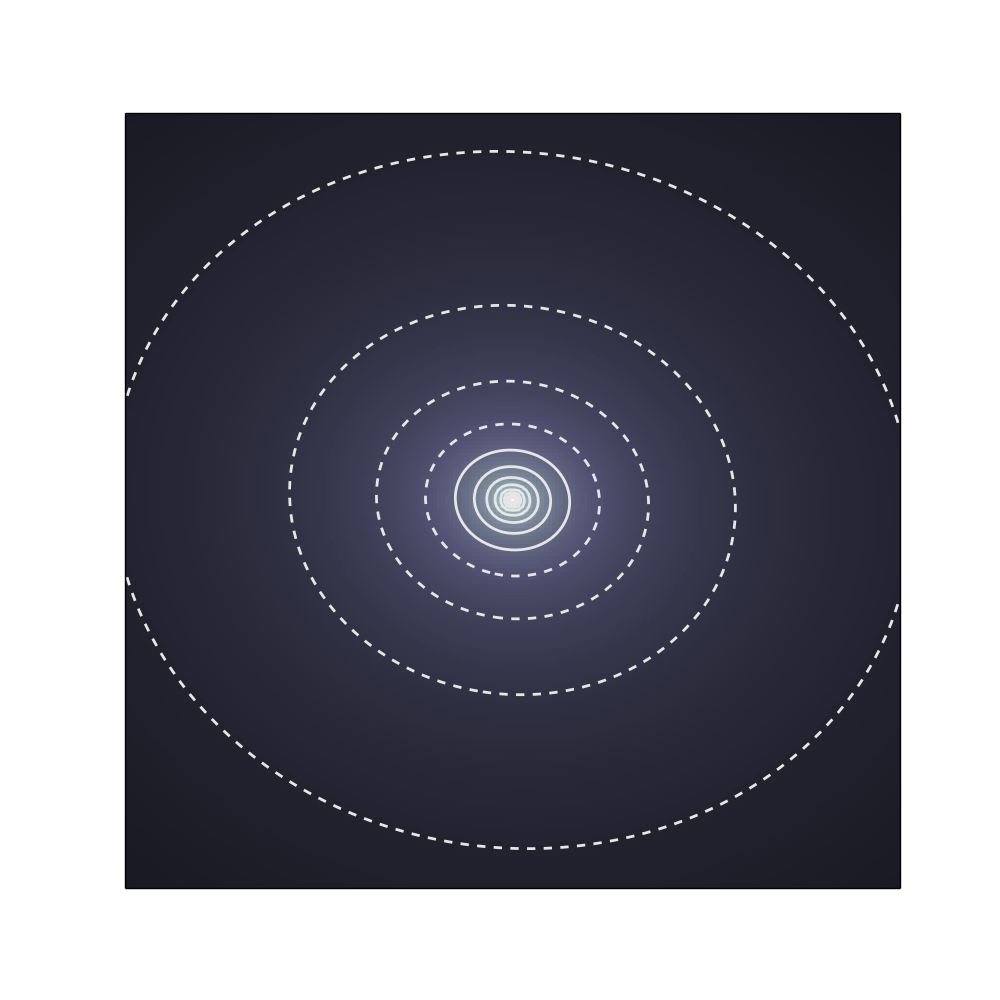
\includegraphics[width=0.45\textwidth]{fig/ASW000102p_kappa}
%   }
%   \subfigure[real arrival-time surface]{
%     \label{fig:6941_sim_arr}
%     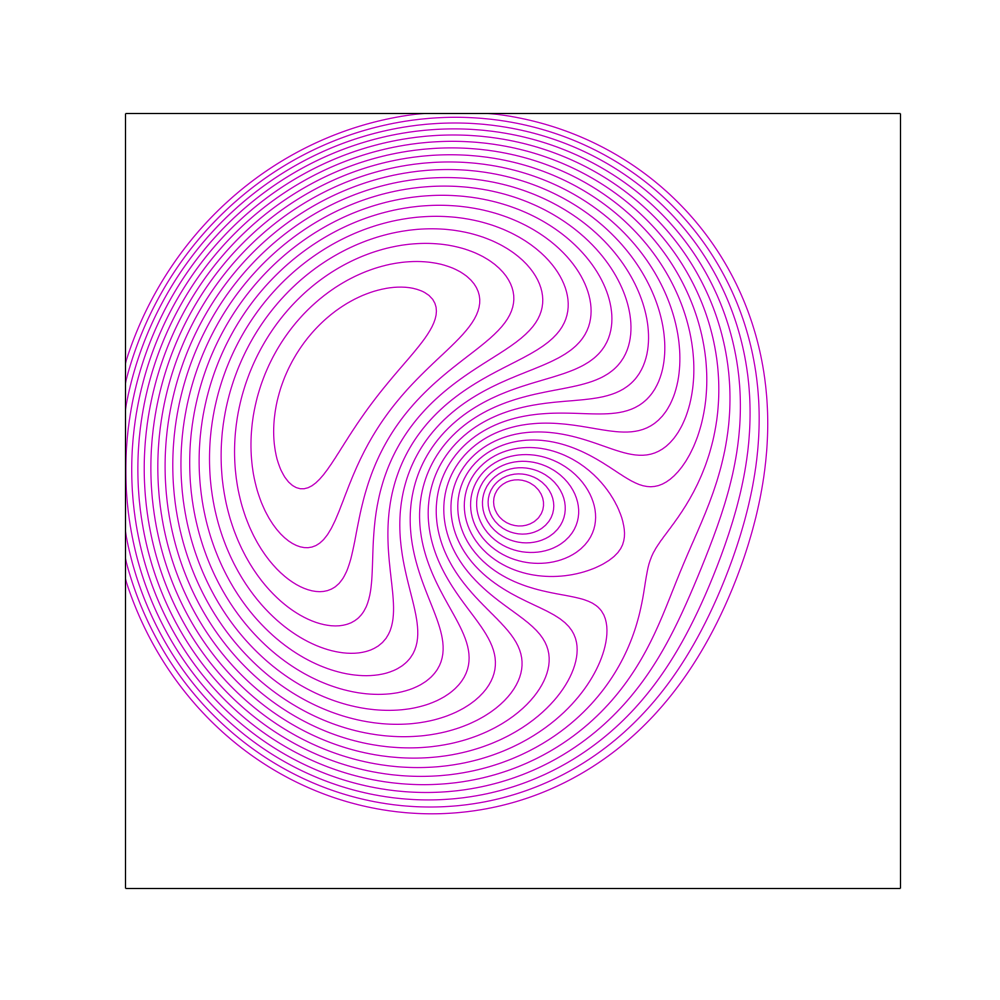
\includegraphics[width=0.45\textwidth]{fig/ASW000102p_arriv}
%   }
%   \subfigure[model mass distribution]{
%     \label{fig:6941_mass}
%     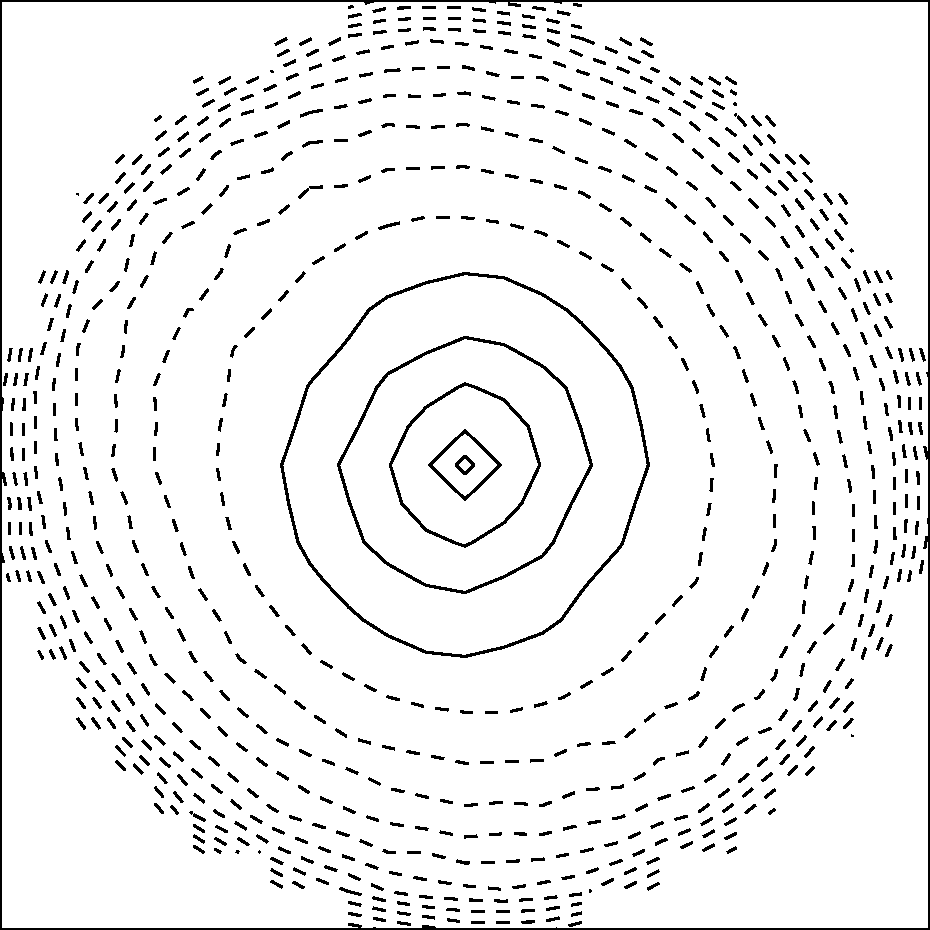
\includegraphics[width=0.45\textwidth]{fig/006941_mass}
%   }
%   \subfigure[model arrival-time surface]{
%     \label{fig:6941_cont}
%     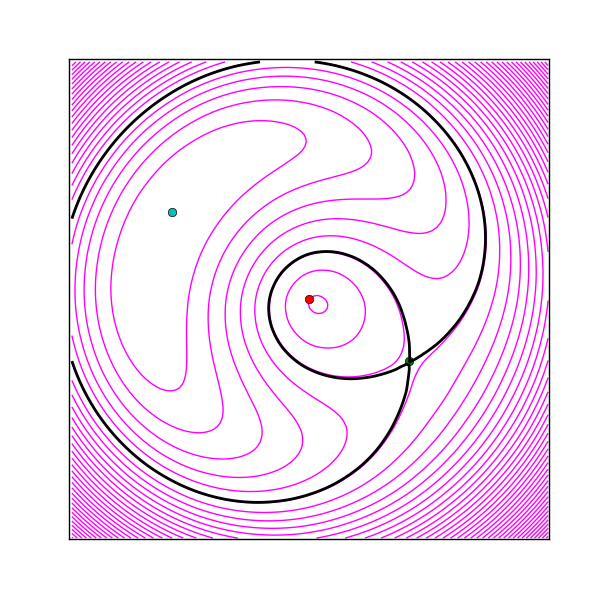
\includegraphics[width=0.45\textwidth]{fig/006941_spaghetti}
%   }
%   \subfigure[real vs model enclosed mass]{
%     \label{fig:6941_kappa}
%     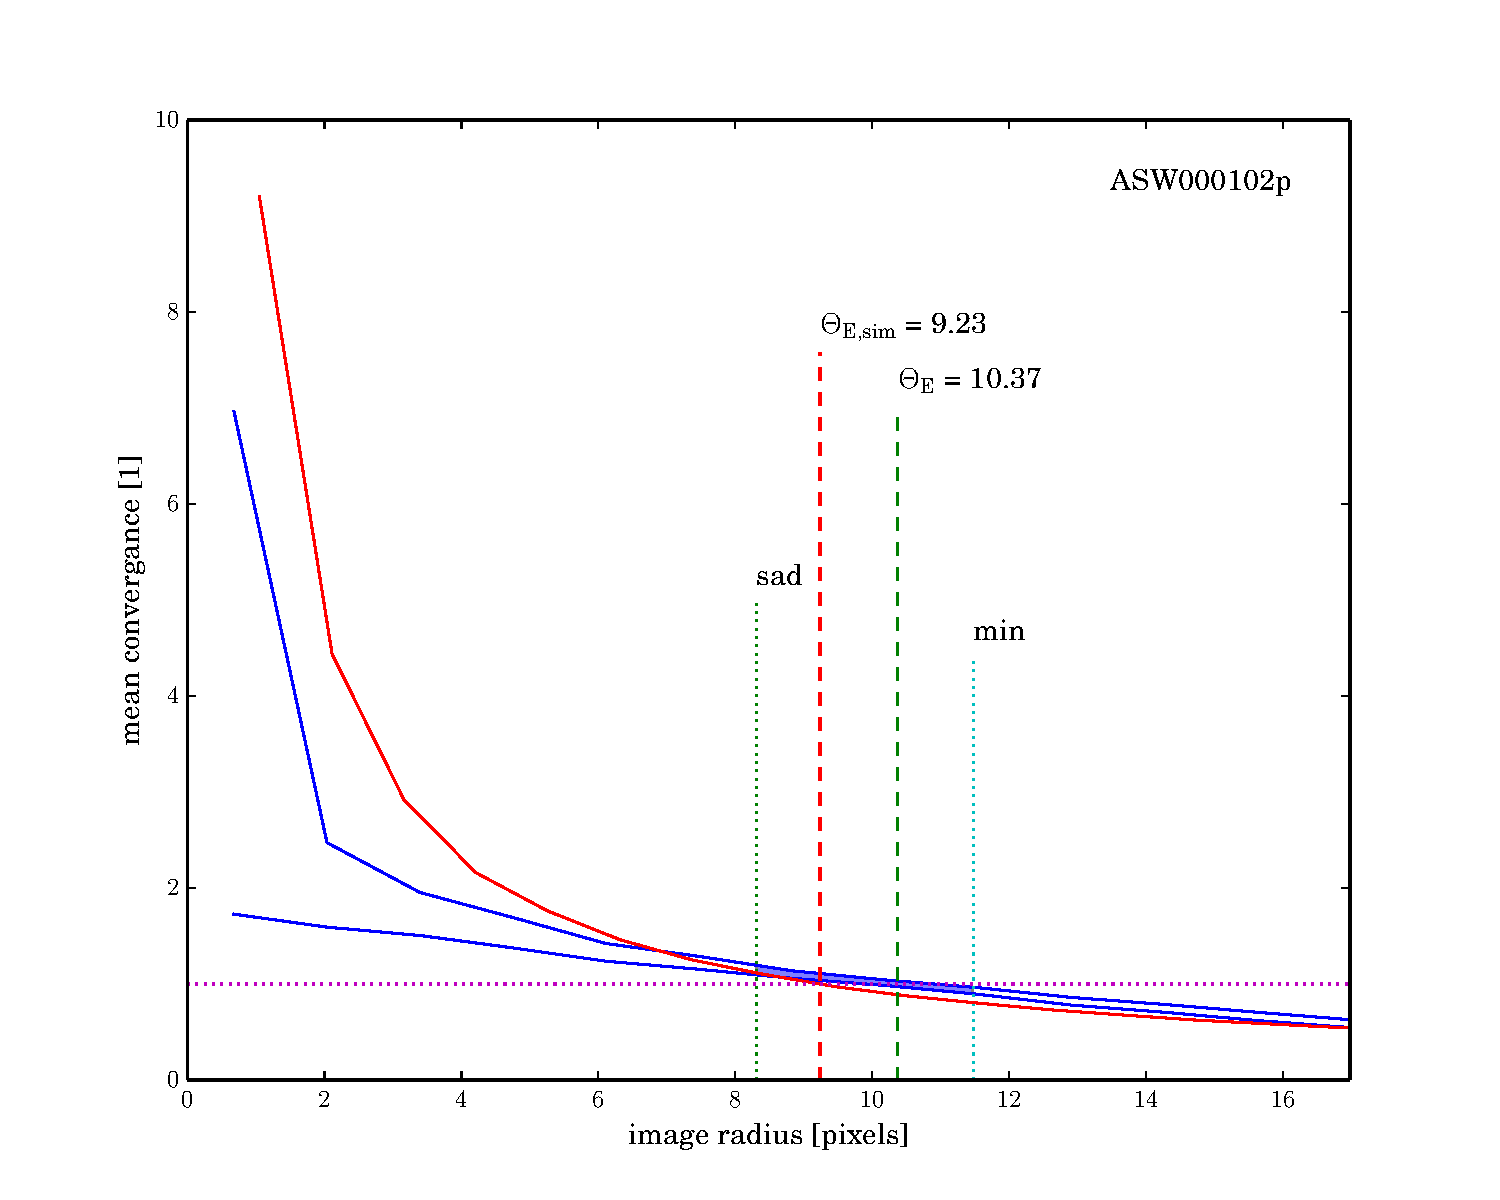
\includegraphics[width=0.45\textwidth]{fig/006941_kappa_encl}
%   }
%   \subfigure[model lensed image]{
%     \label{fig:6941_atime}
%     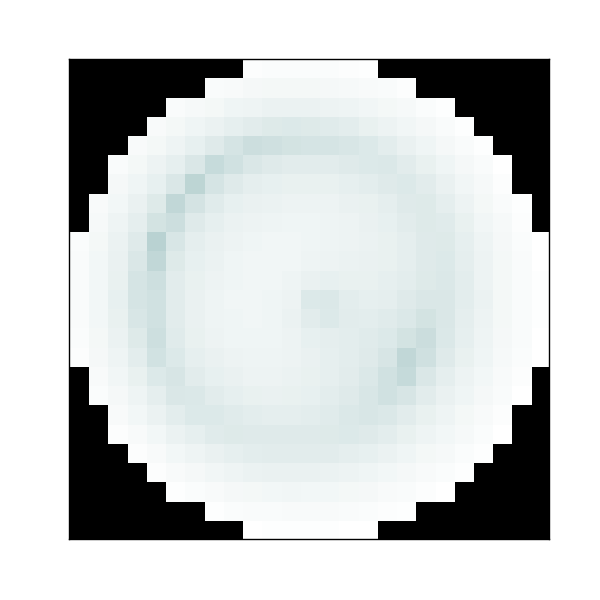
\includegraphics[width=0.45\textwidth]{fig/006941_arr_time}
%   }
%   \caption[result 6941 (ASW000102p)]{Model results for a simple
%     simulated lens.  (The label ASW000102p in the lower-left panel is
%     the \sw identifier for the sky patch where this sim was placed.)
%     The model input is shown in the top panel of
%     Figure~\ref{fig:input-spag}.  For details of the individual panels
%     here, see section \ref{sec:example_models}.}
%   \label{fig:6941}
% \end{figure}

% Rafik's two row design

\newpage

\begin{figure}
  \centering
  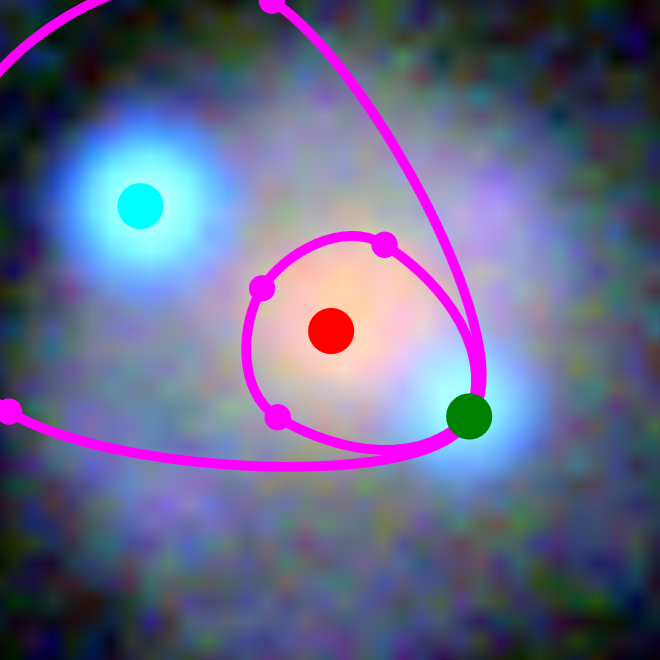
\includegraphics[width=\myplotswidth]{fig/006941_input}
  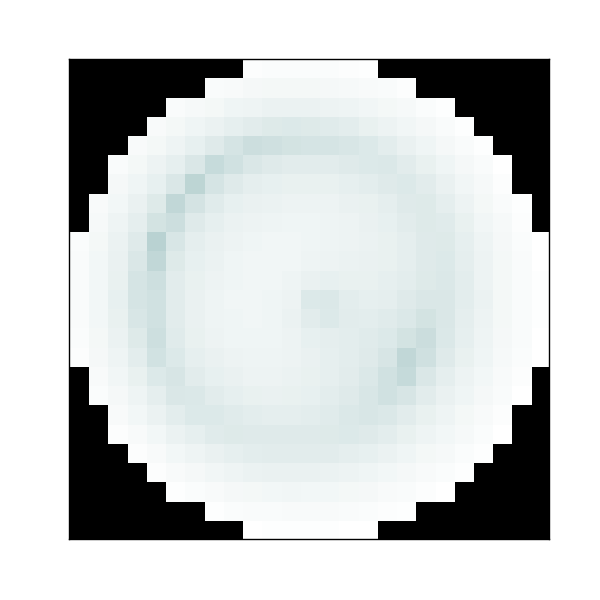
\includegraphics[width=\myplotswidth]{fig/006941_arr_time} \\
  \vskip-20pt
  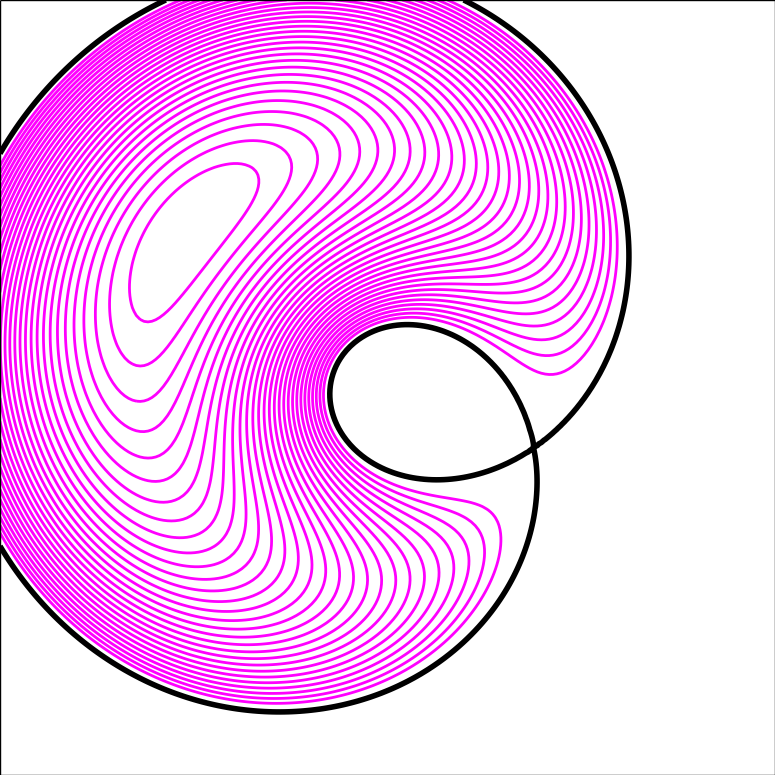
\includegraphics[width=\myplotswidth]{fig/ASW000102p_006941_arriv} 
  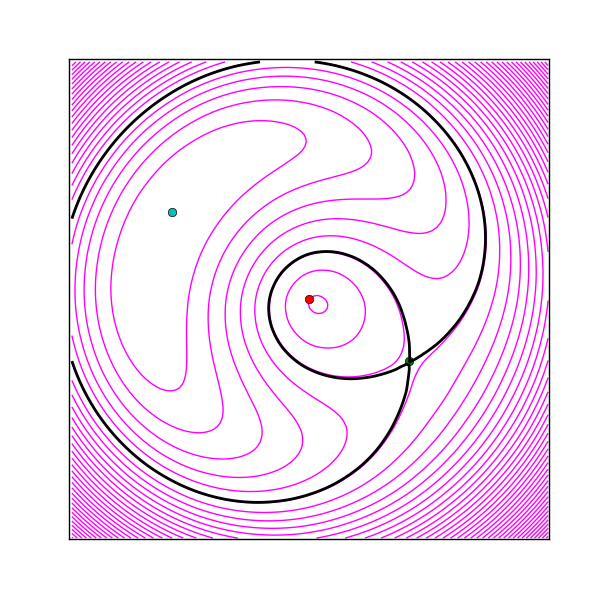
\includegraphics[width=\myplotswidth]{fig/006941_spaghetti} \\
  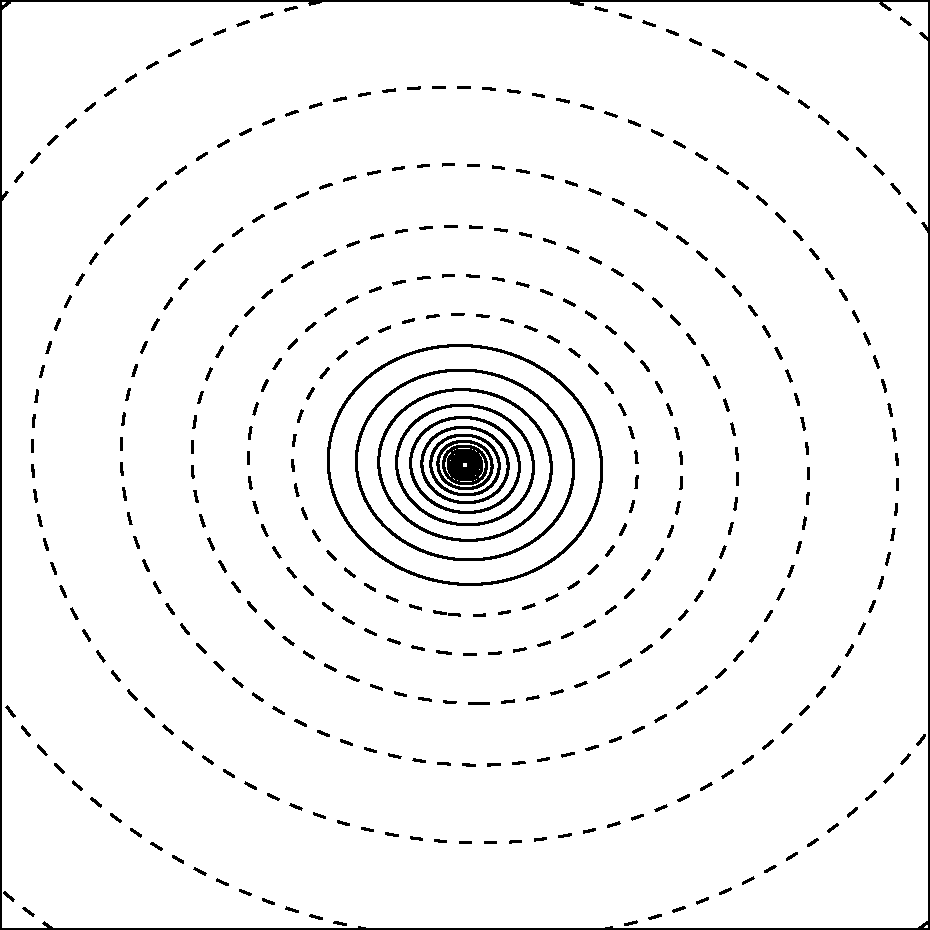
\includegraphics[width=\myplotswidth]{fig/ASW000102p_006941_kappa}
  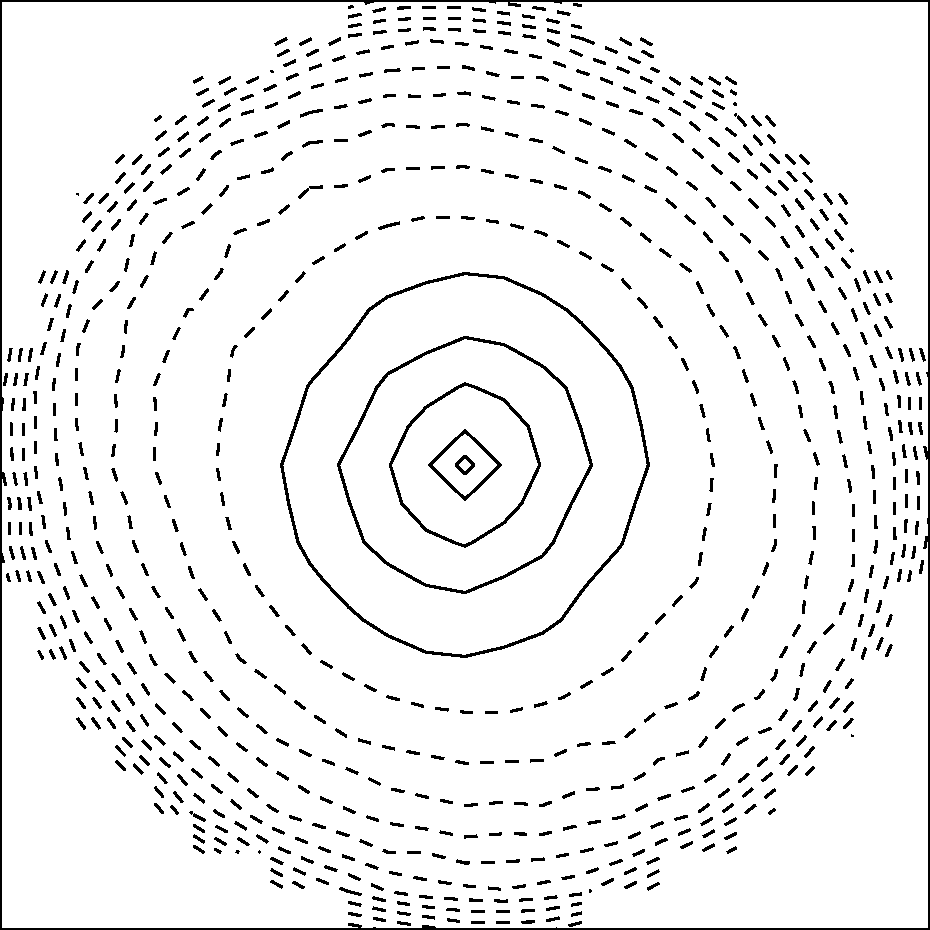
\includegraphics[width=\myplotswidth]{fig/006941_mass}
  \caption[result 6941 (ASW000102p)]{A simulated lens that mimics a
    lensed quasar, and model results.  The left panels derive from the
    simulation, and the right panels are \sl output.  Details of
    individual panels are in \ref{sec:example_models}.}

  \label{fig:6941}
\end{figure}

\begin{figure}
  \centering

  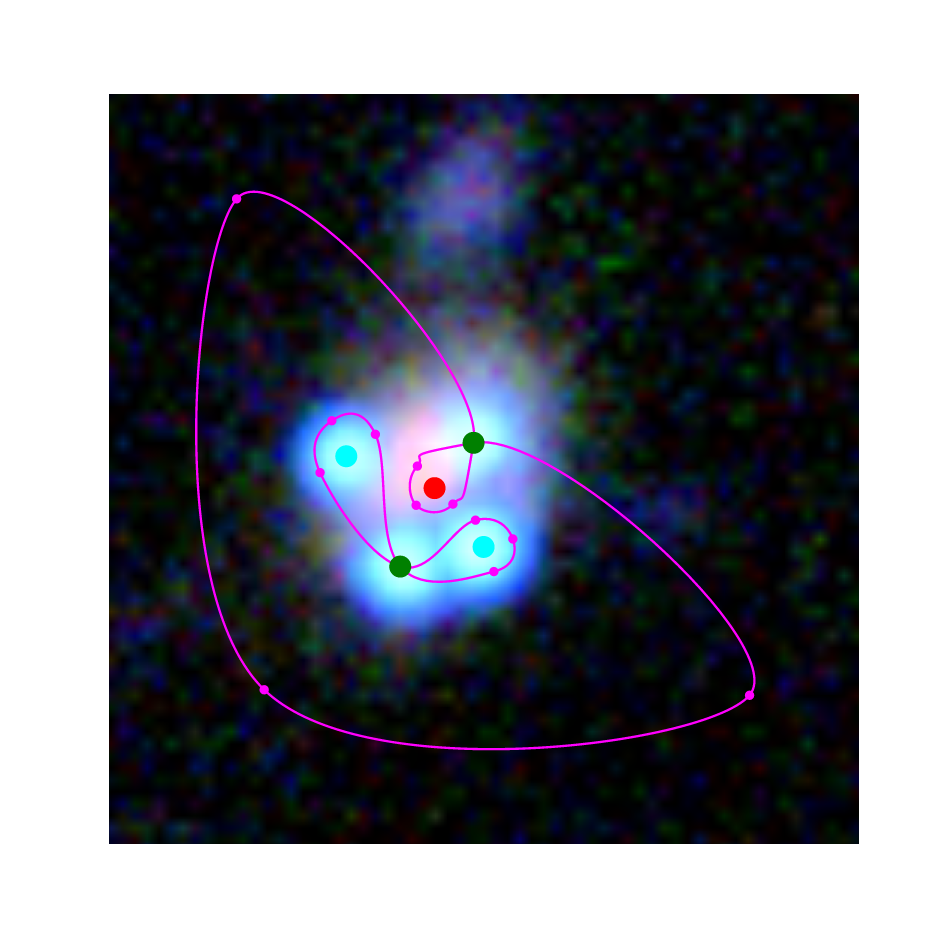
\includegraphics[width=\myplotswidth]{fig/006915_input}
  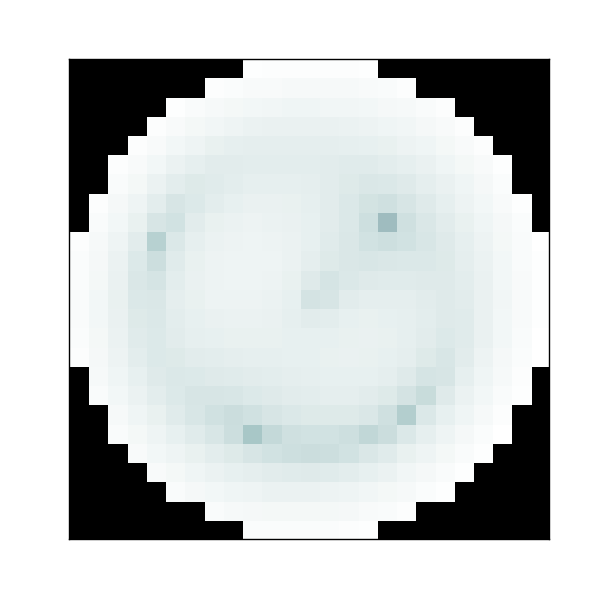
\includegraphics[width=\myplotswidth]{fig/006915_arr_time} \\
  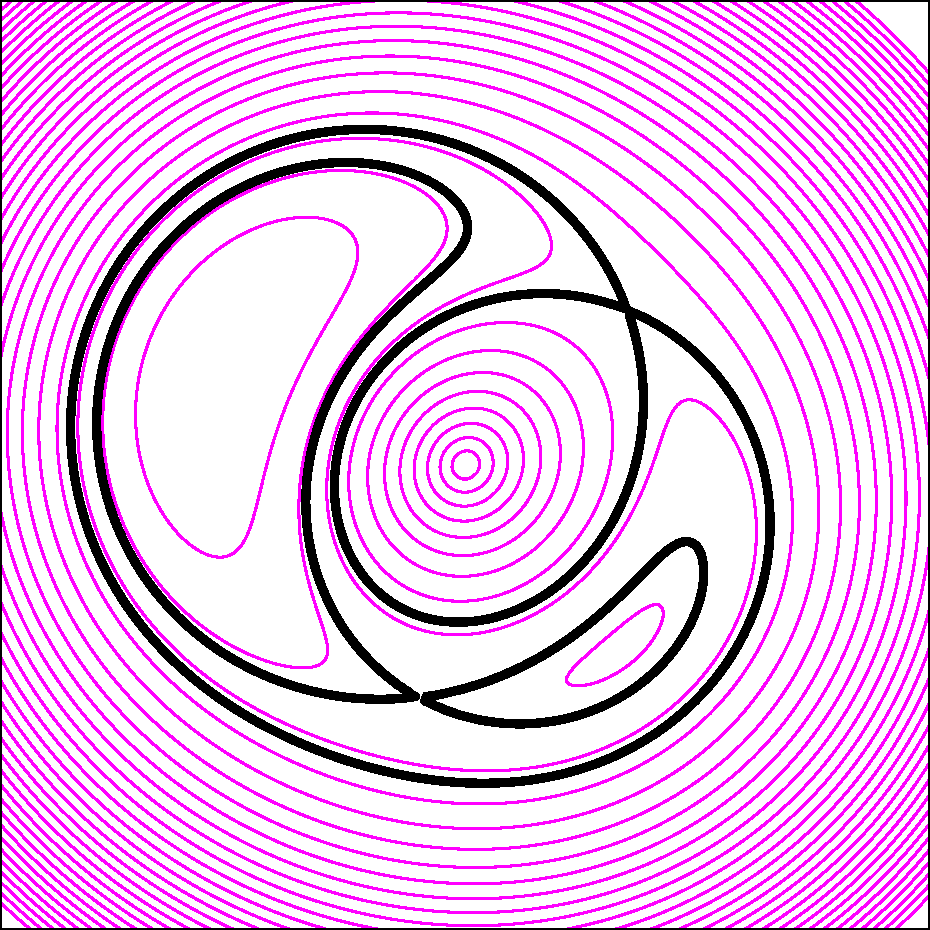
\includegraphics[width=\myplotswidth]{fig/ASW0001hpf_006915_arriv}
  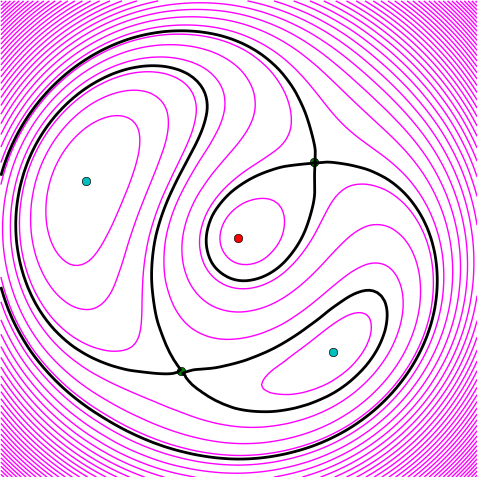
\includegraphics[width=\myplotswidth]{fig/006915_spaghetti} \\
  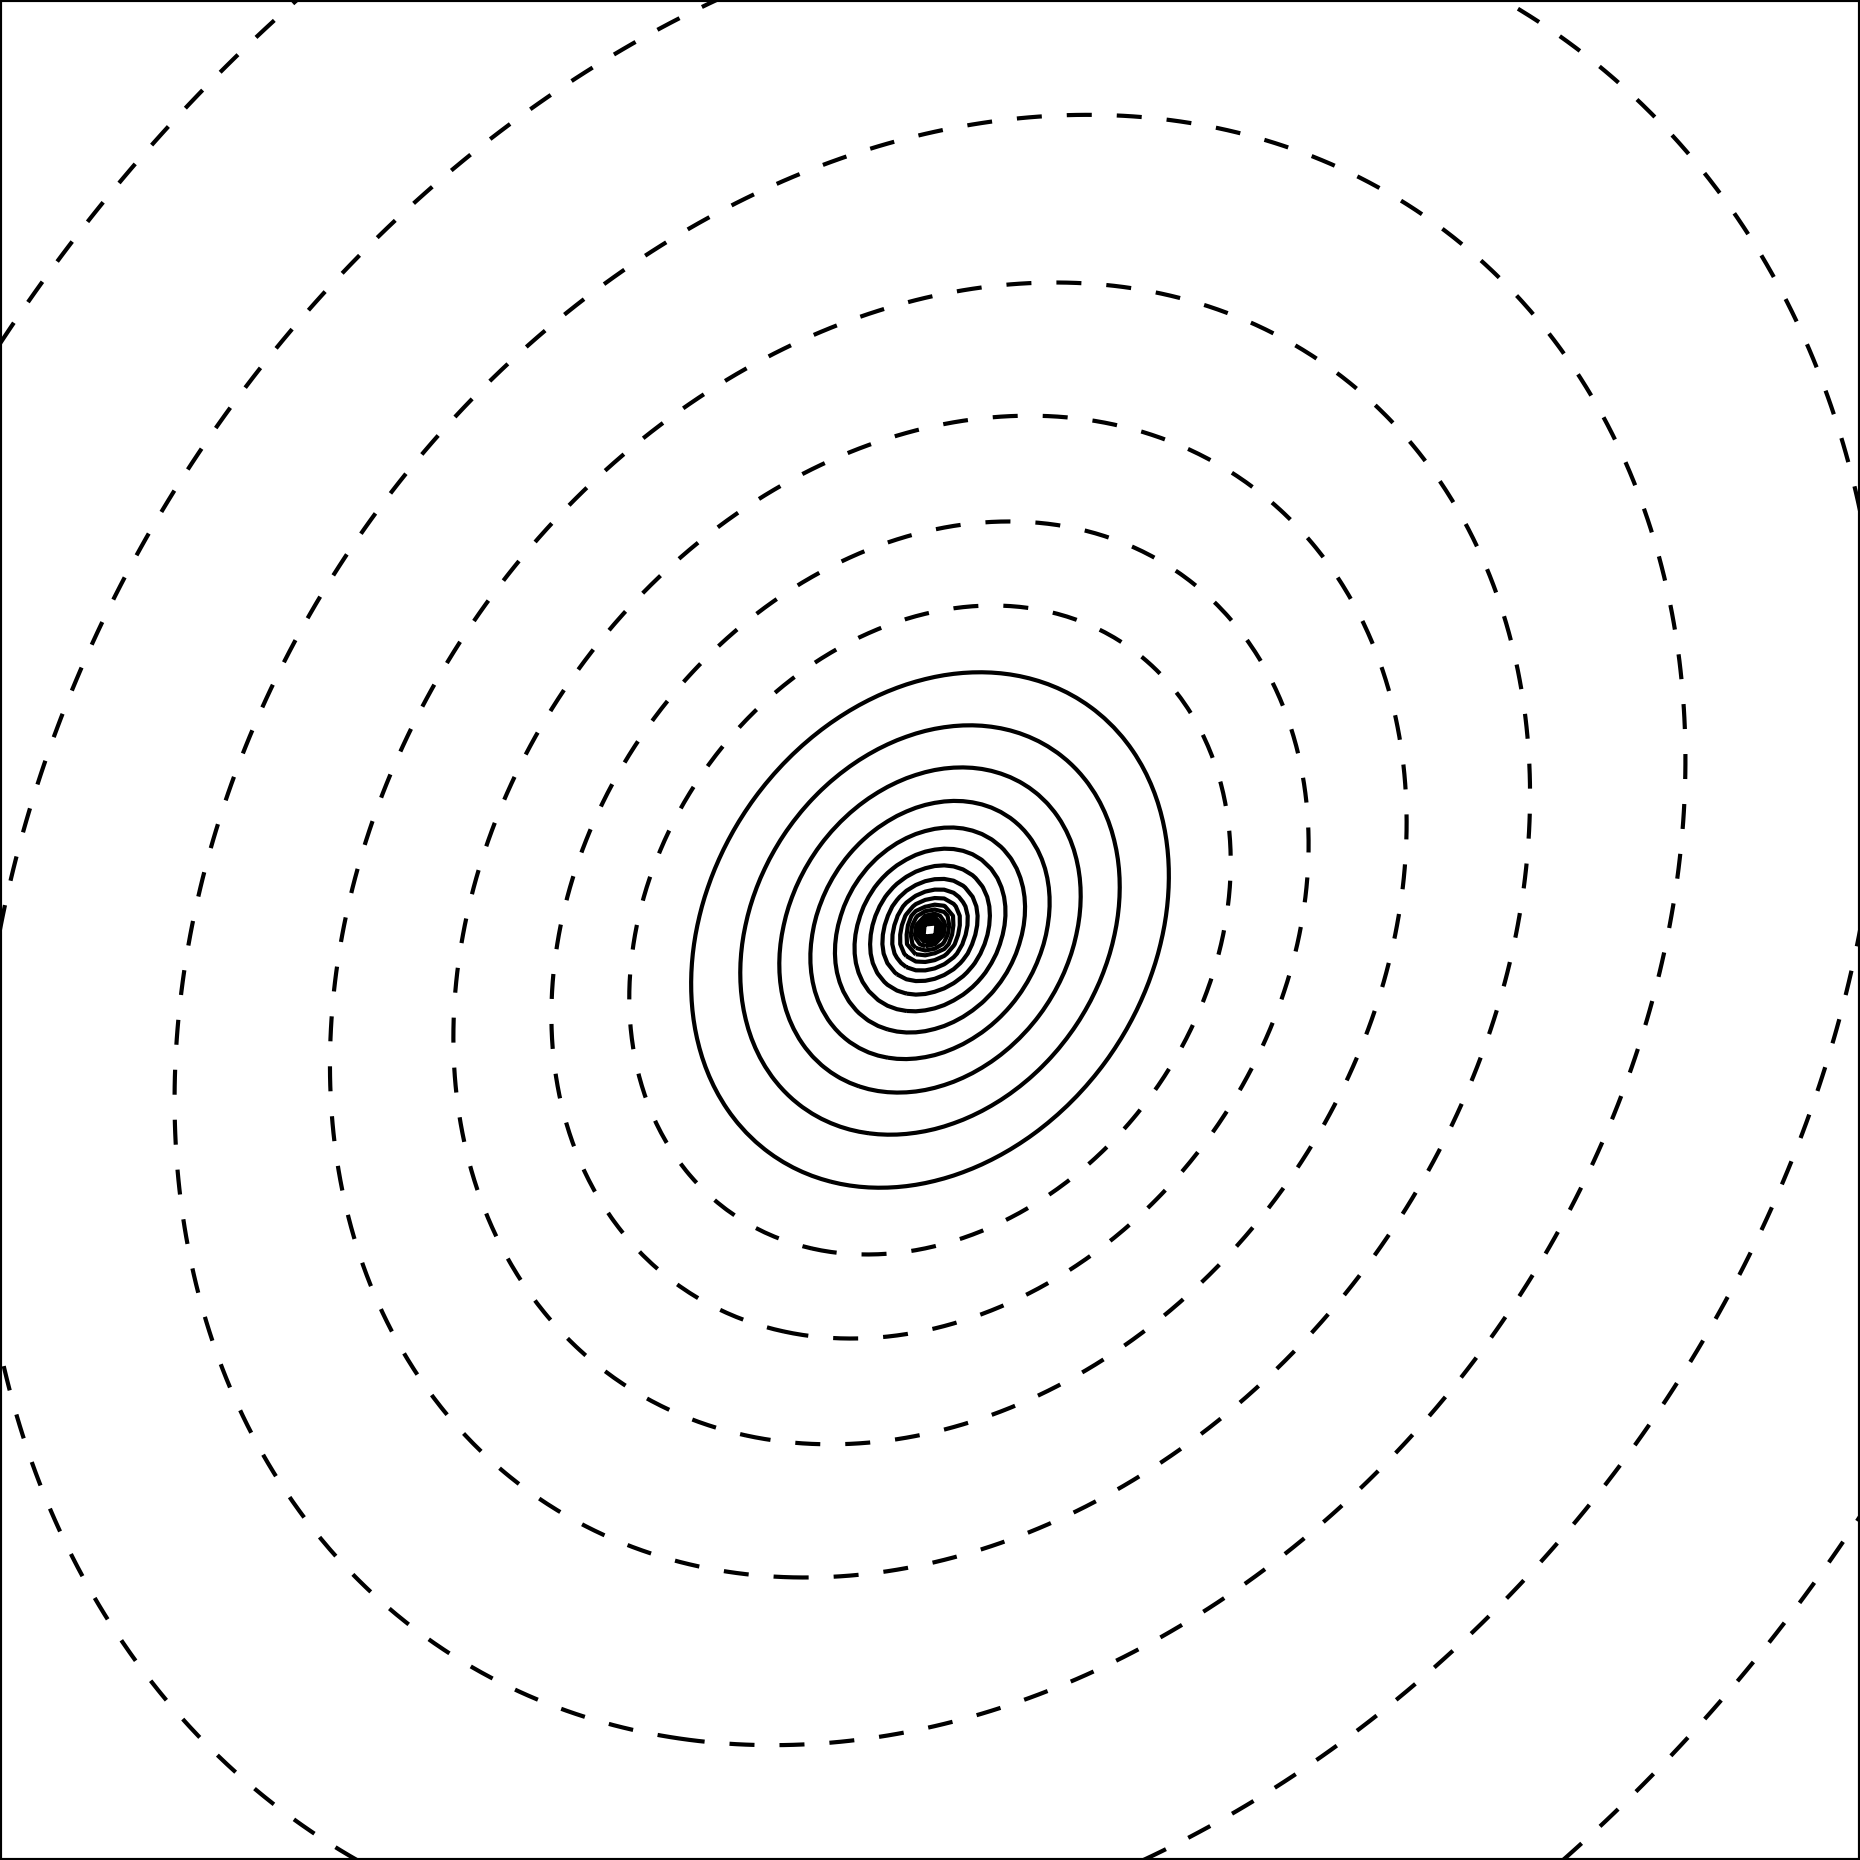
\includegraphics[width=\myplotswidth]{fig/ASW0001hpf_006915_kappa}
  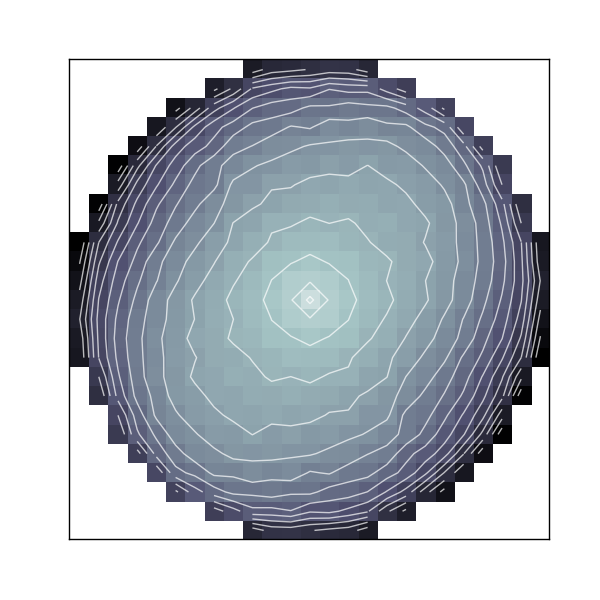
\includegraphics[width=\myplotswidth]{fig/006915_mass}

  \caption[result 6915 (ASW0001hpf)]{A four-image configuration
    typical of lensed quasars. (See Section \ref{sec:example_models}
    for details.)}
  \label{fig:6915}
\end{figure}






\begin{figure}
  \centering
  
  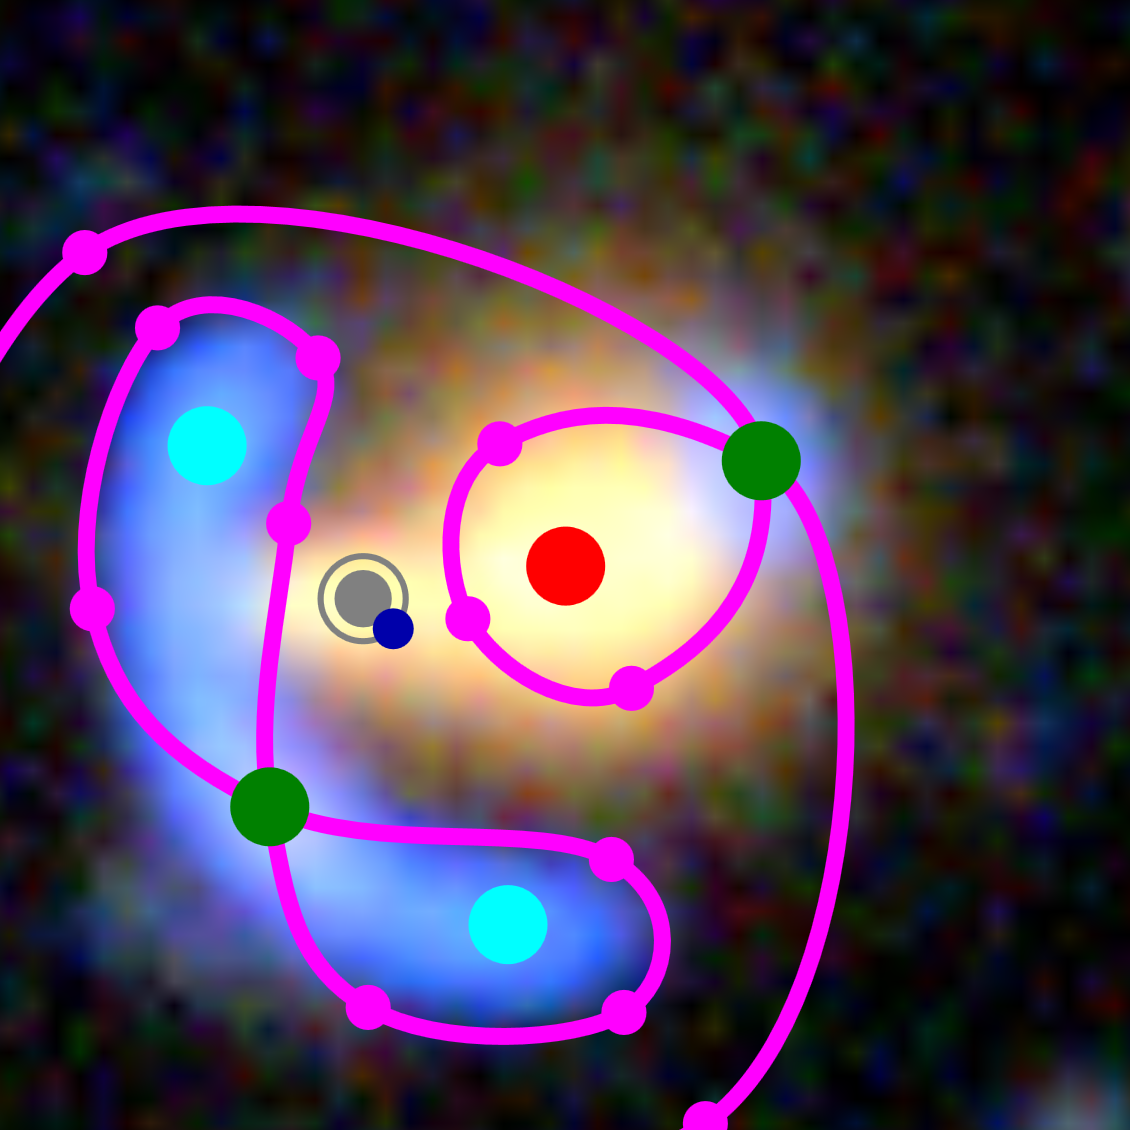
\includegraphics[width=\myplotswidth]{fig/006990_input}
  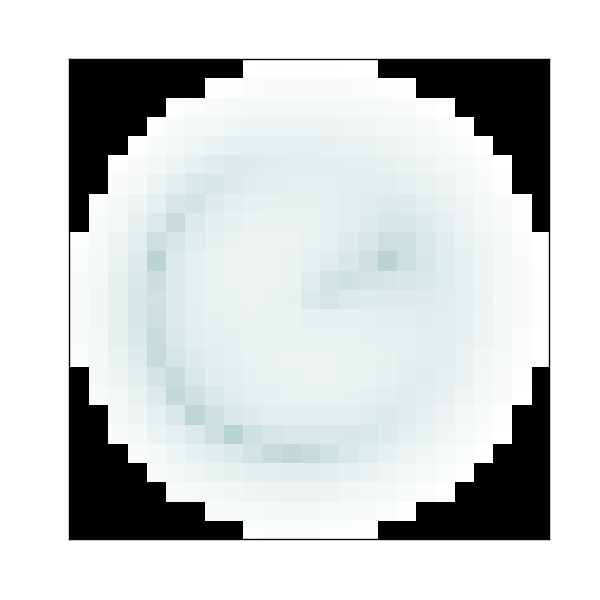
\includegraphics[width=\myplotswidth]{fig/006990_arr_time} \\
  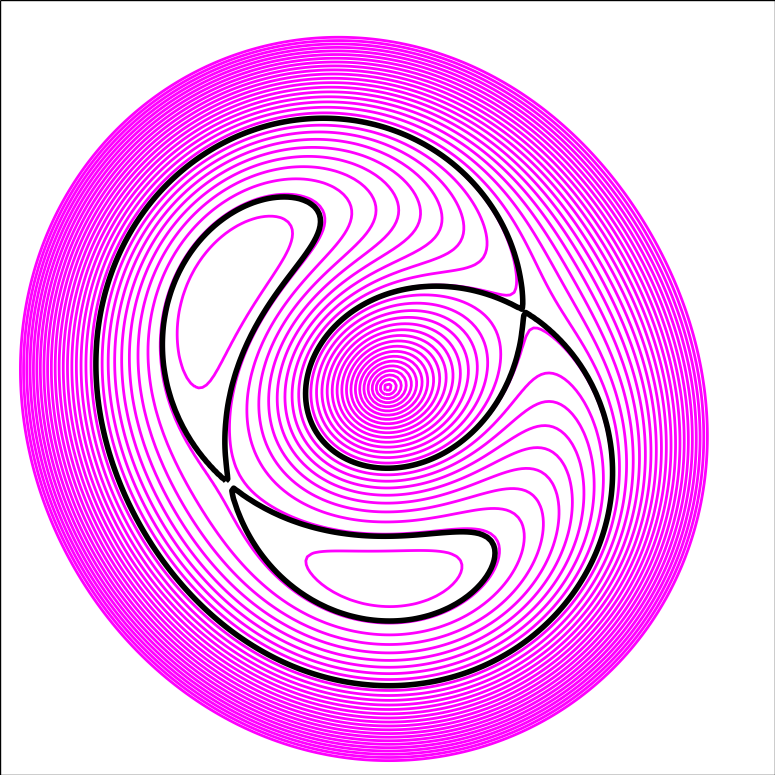
\includegraphics[width=\myplotswidth]{fig/ASW0004oux_006990_arriv}
  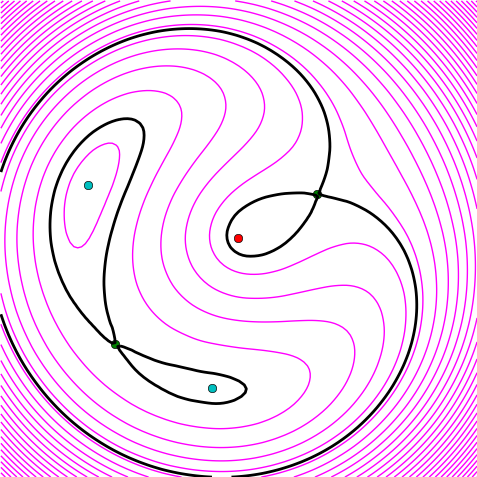
\includegraphics[width=\myplotswidth]{fig/006990_spaghetti} \\
  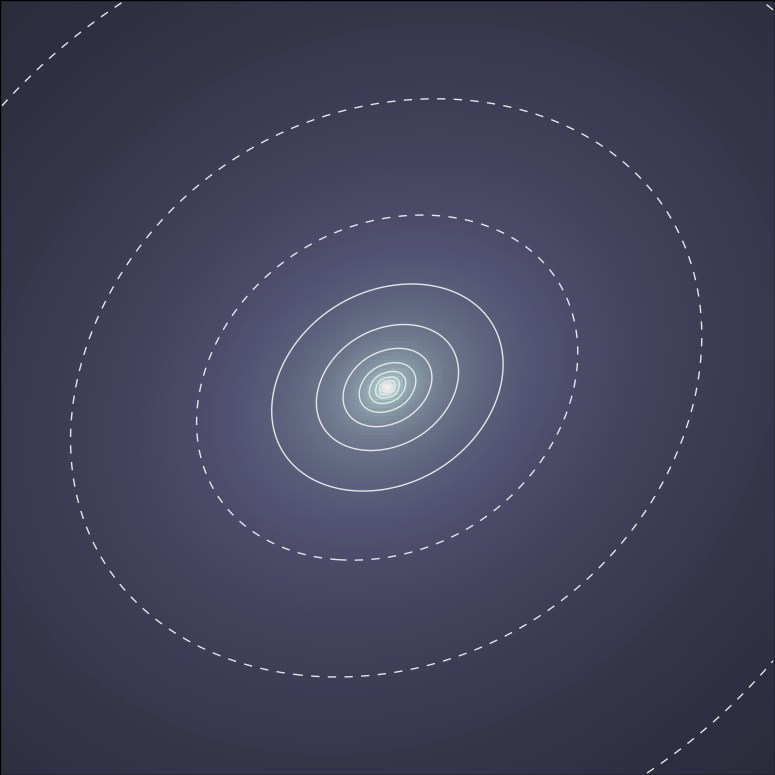
\includegraphics[width=\myplotswidth]{fig/ASW0004oux_006990_kappa}
  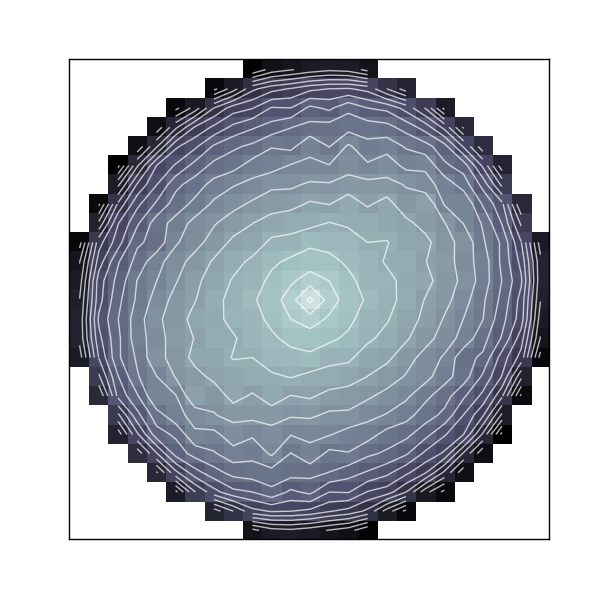
\includegraphics[width=\myplotswidth]{fig/006990_mass}

  \caption[result 6990 (ASW0004oux)]{Results from a system with an arc
    plus a counter-image, typical of lensed galaxies. (See Section
    \ref{sec:example_models} for details.)}
  \label{fig:6990}
\end{figure}



\begin{figure}
  \centering

  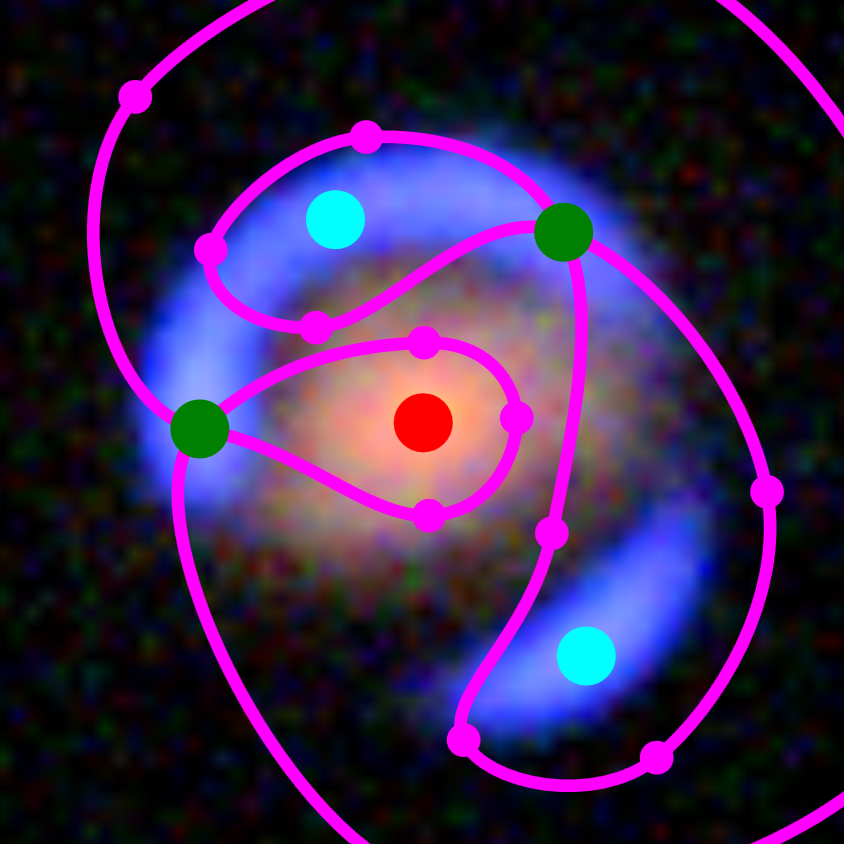
\includegraphics[width=\myplotswidth]{fig/006919_input}
  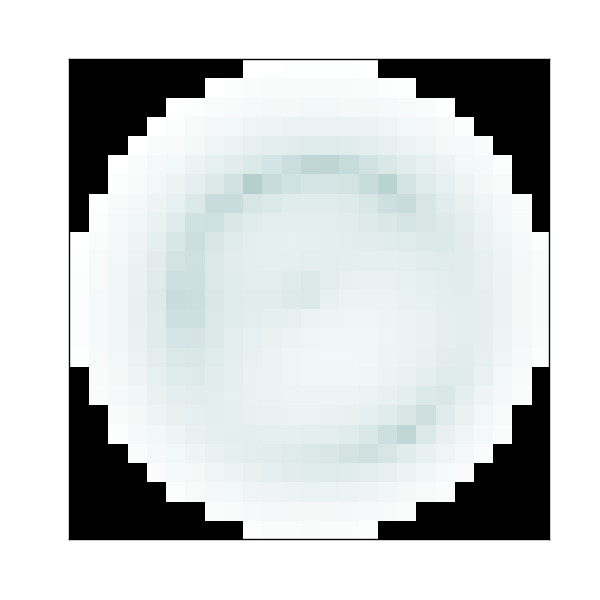
\includegraphics[width=\myplotswidth]{fig/006919_arr_time} \\
  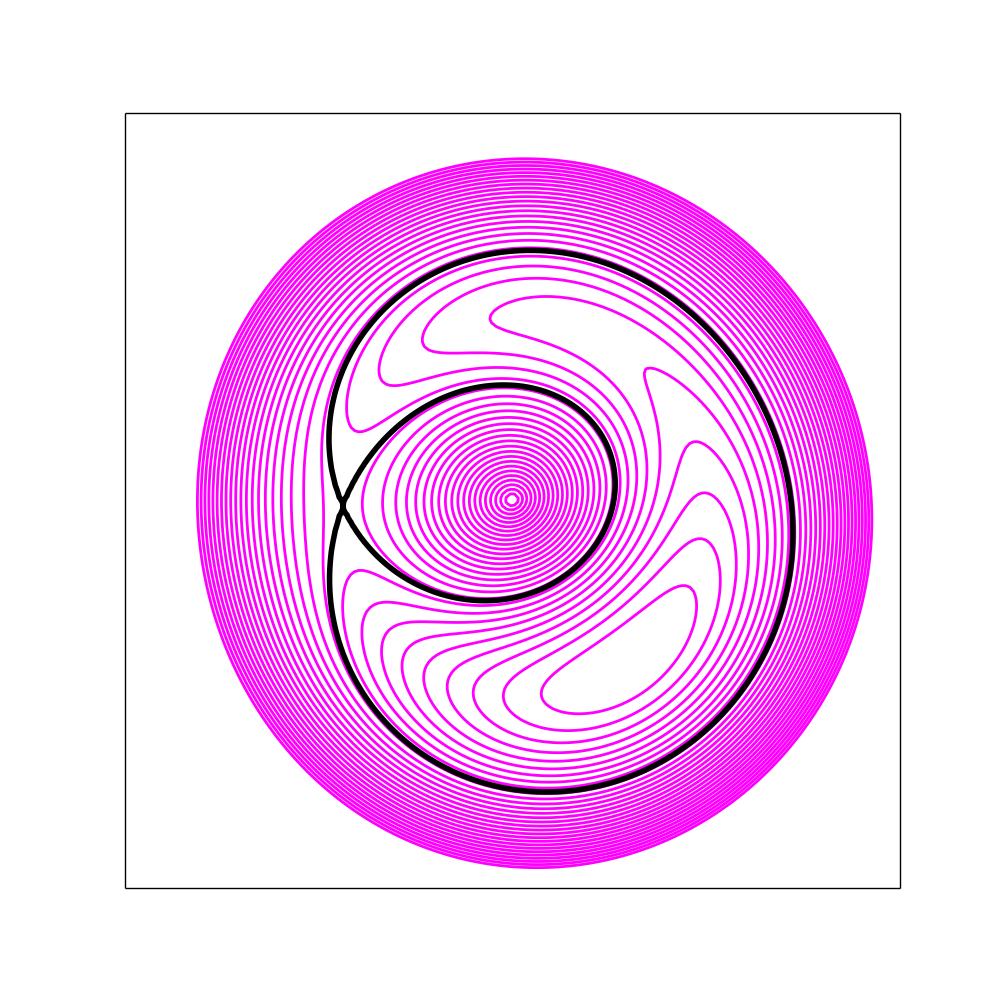
\includegraphics[width=\myplotswidth]{fig/ASW0002z6f_006919_arriv}
  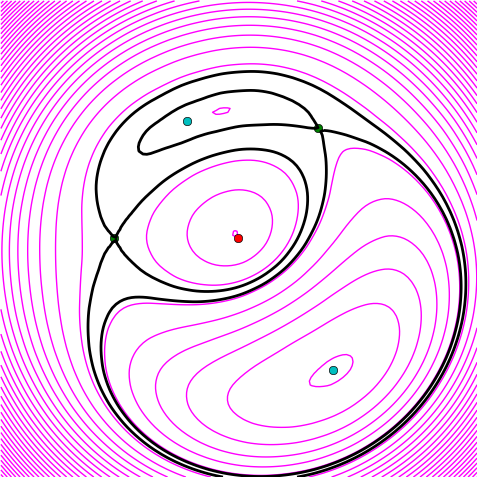
\includegraphics[width=\myplotswidth]{fig/006919_spaghetti} \\
  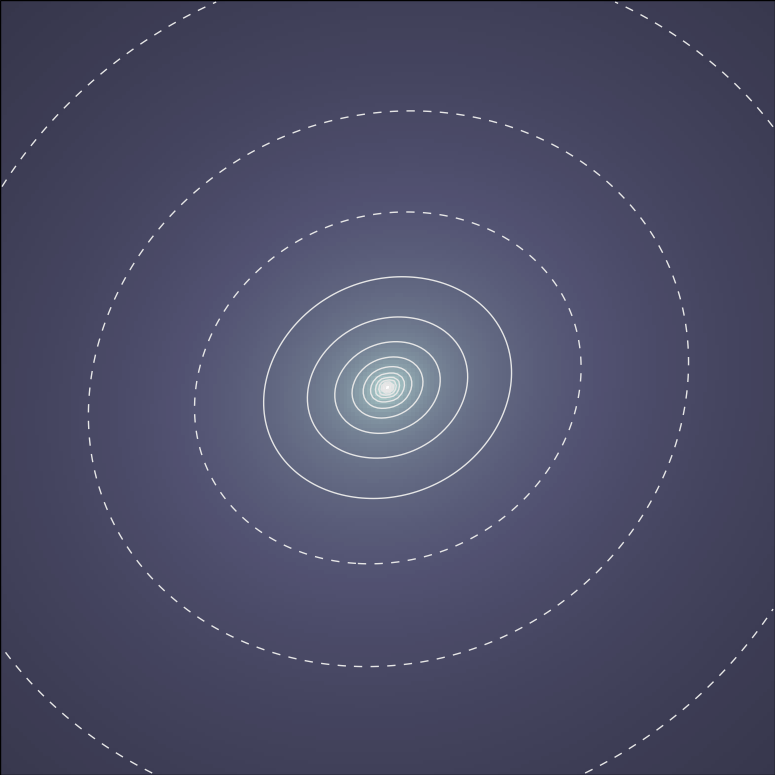
\includegraphics[width=\myplotswidth]{fig/ASW0002z6f_006919_kappa}
  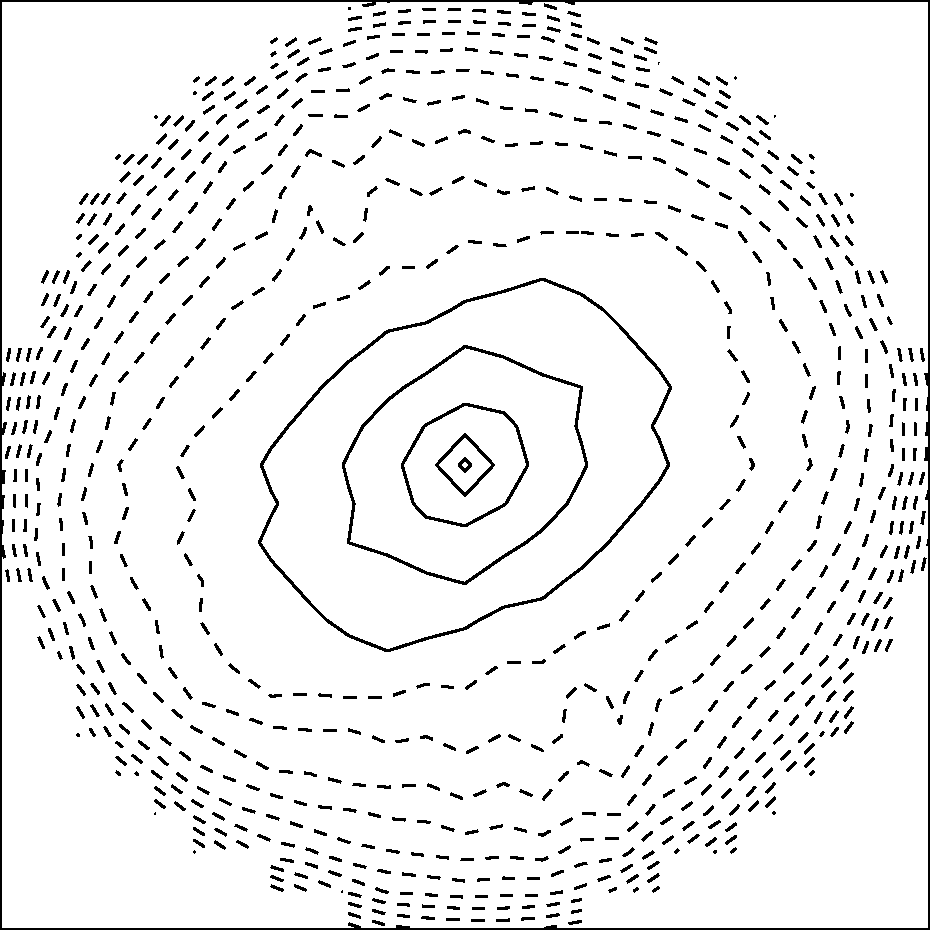
\includegraphics[width=\myplotswidth]{fig/006919_mass}

  \caption[result 6919 (ASW0002z6f)]{Another configuration of arc plus
    counter-image; here the arc is closer to the lensing galaxy than
    the counter-image. (See Section \ref{sec:example_models} for
    details.)}
  \label{fig:6919}
\end{figure}



\begin{figure}
  \centering
  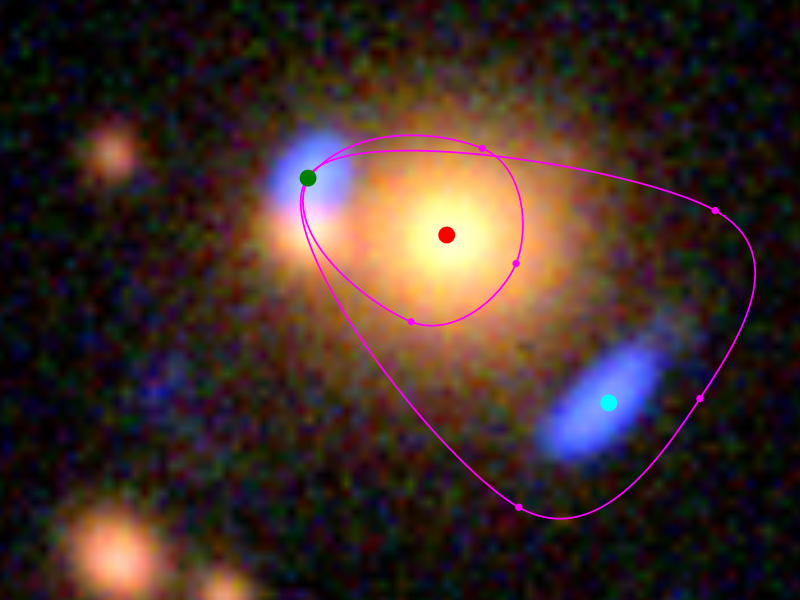
\includegraphics[width=\myplotswidth]{fig/006975_input}
  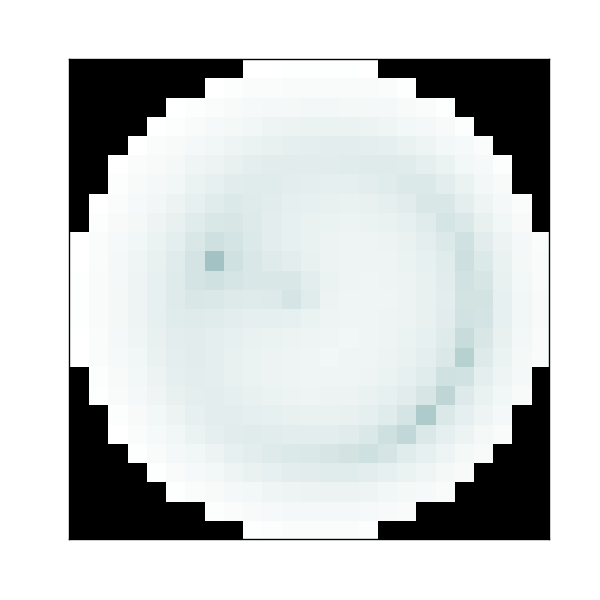
\includegraphics[width=\myplotswidth]{fig/006975_arr_time} \\
  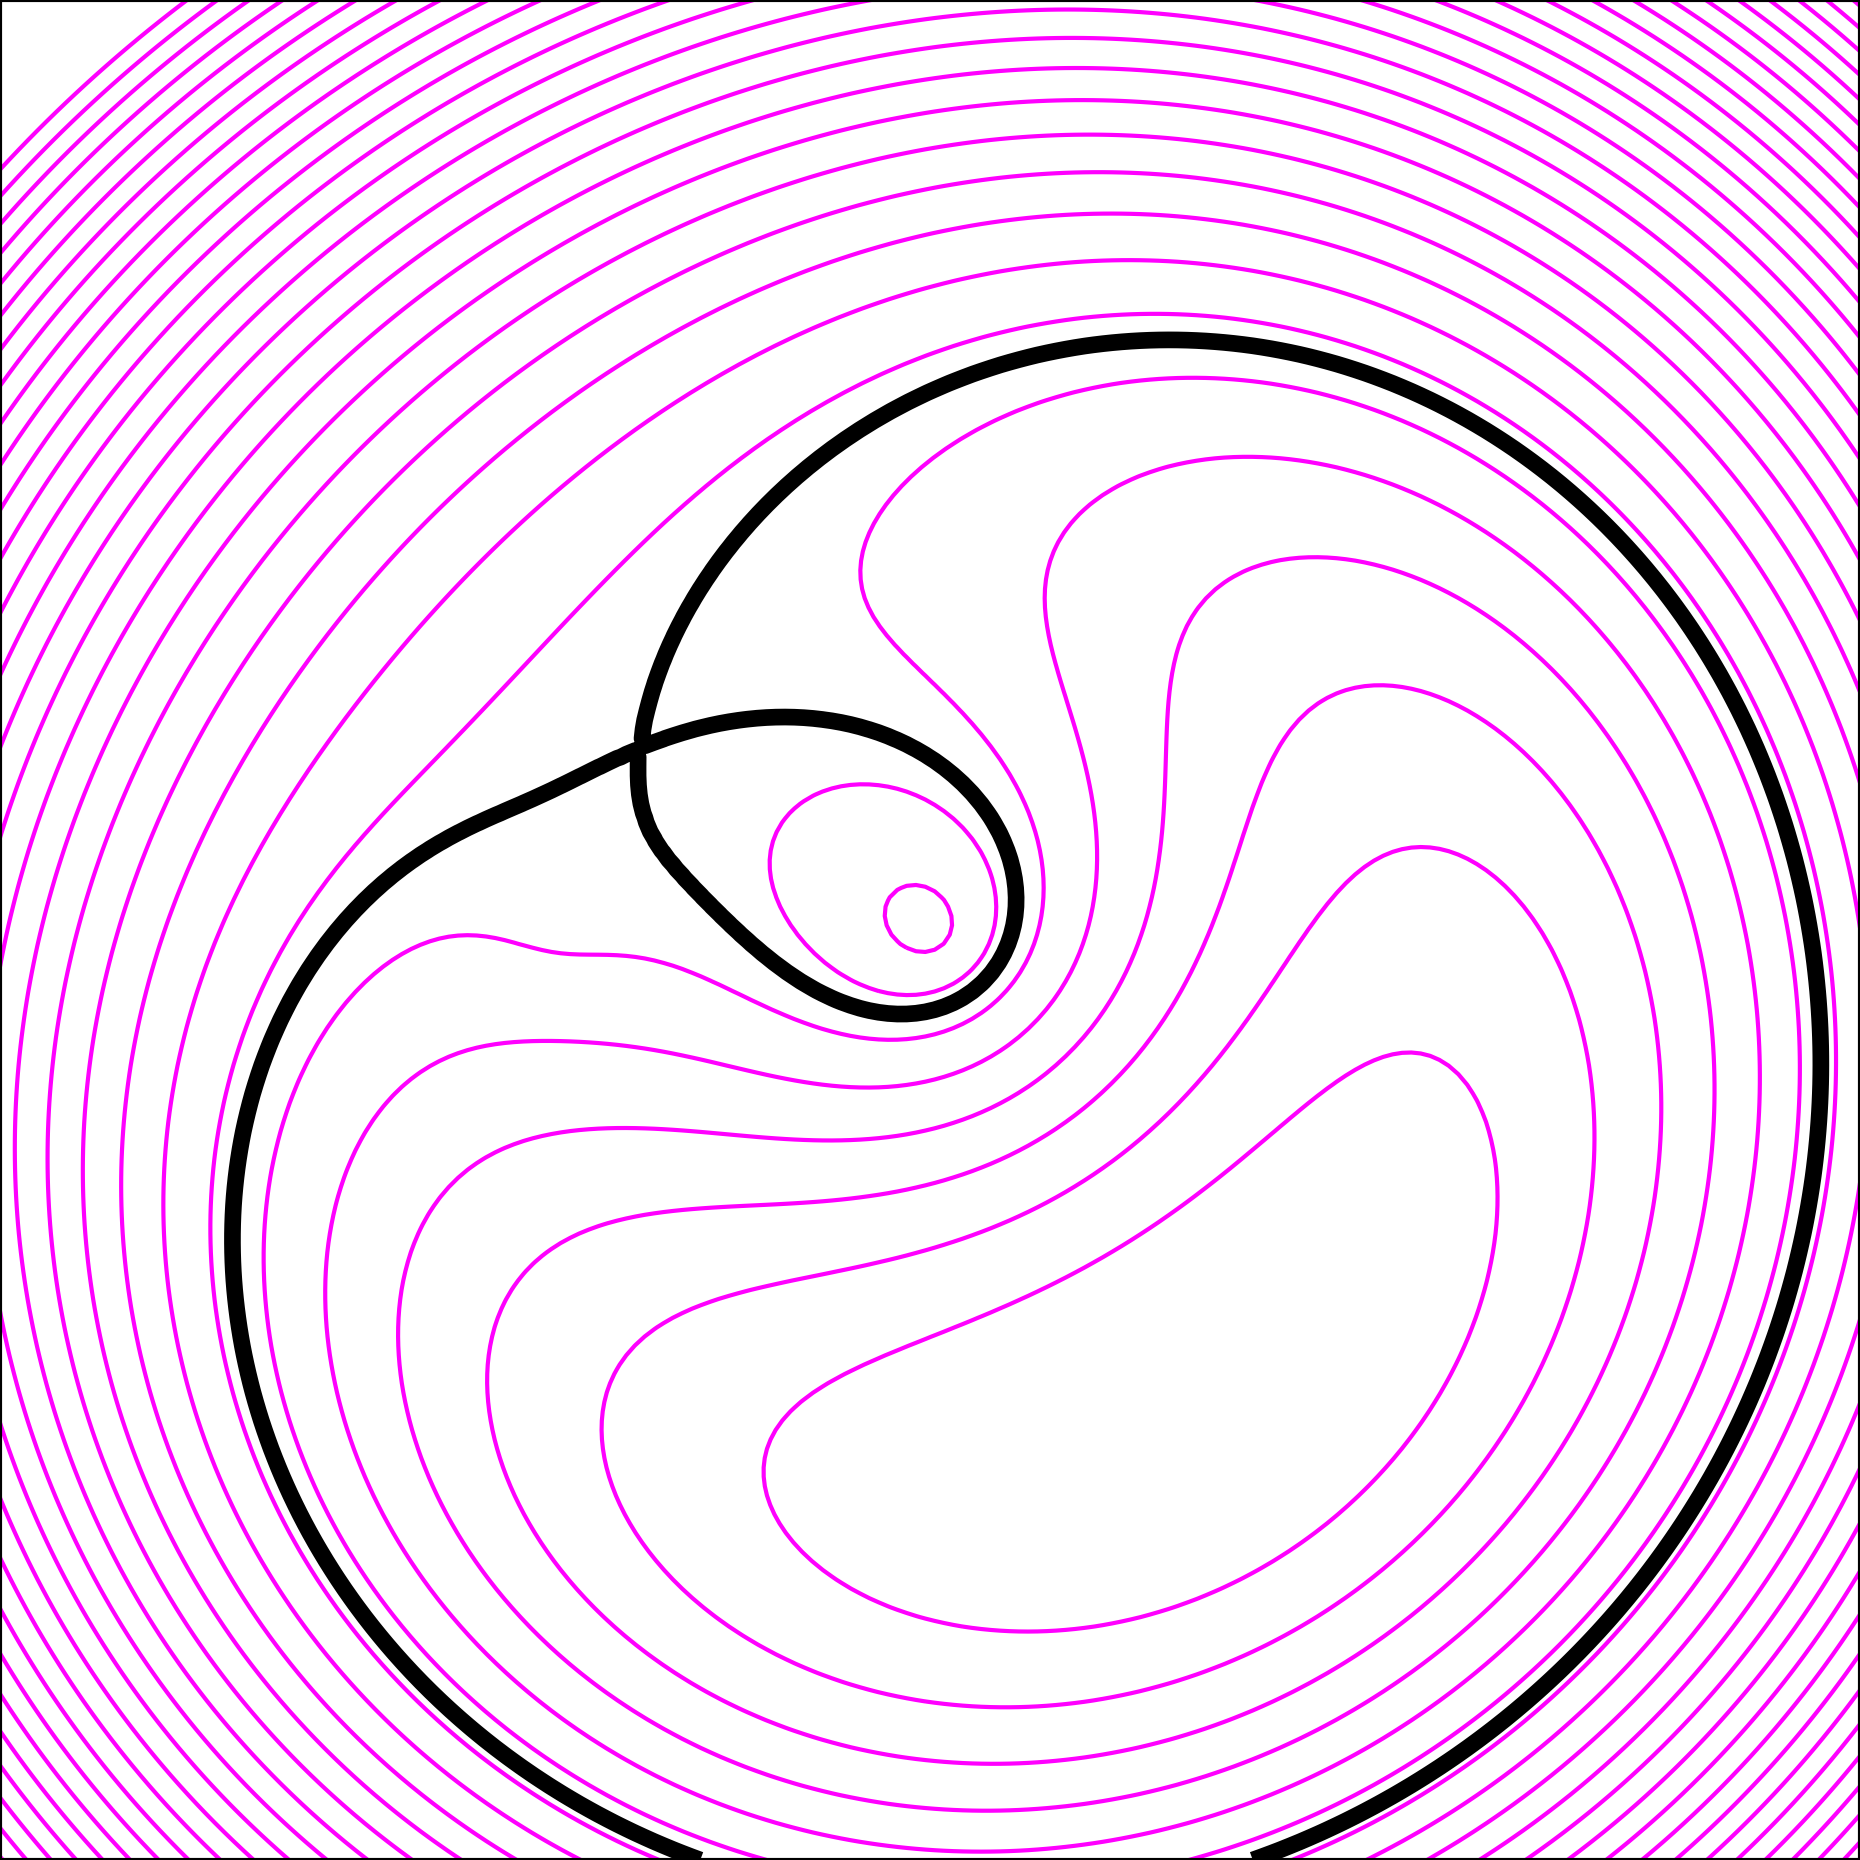
\includegraphics[width=\myplotswidth]{fig/ASW000195x_006975_arriv.png}
  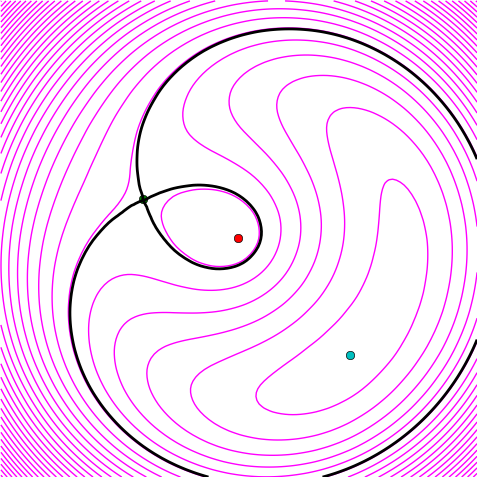
\includegraphics[width=\myplotswidth]{fig/006975_spaghetti} \\
  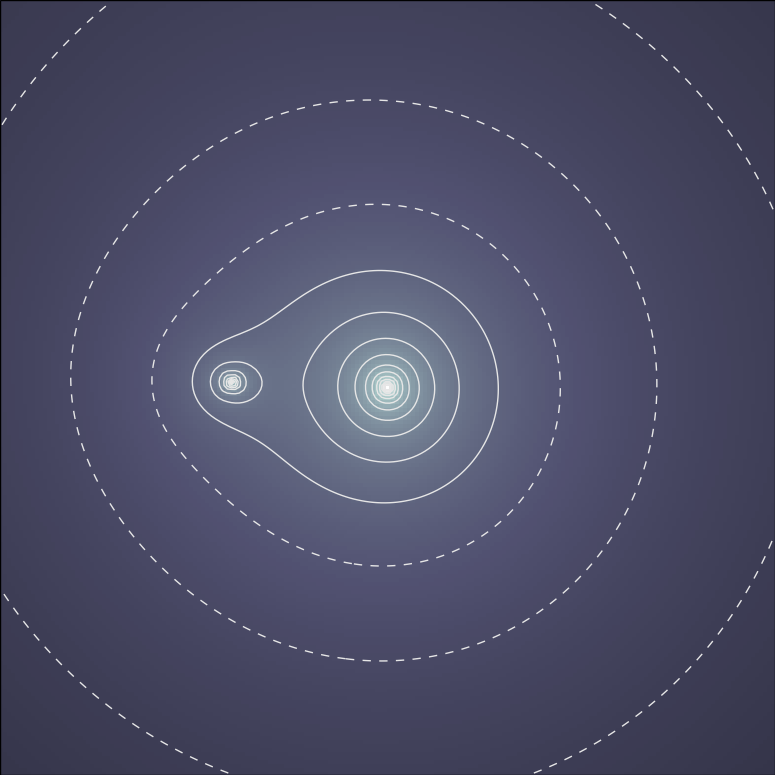
\includegraphics[width=\myplotswidth]{fig/ASW000195x_006975_kappa.png}
  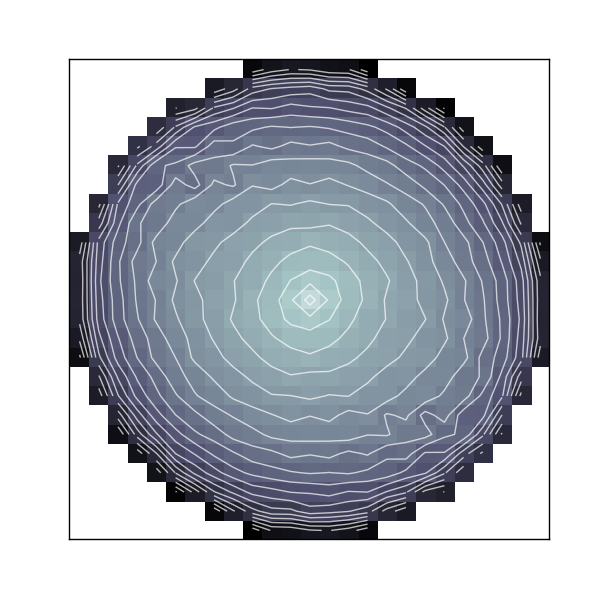
\includegraphics[width=\myplotswidth]{fig/006975_mass}
  \caption[result 6975 (ASW000195x)]{A lens with unrecovered mass
    substructure. (See Section \ref{sec:example_models} for details.)}
  \label{fig:6975}
\end{figure}
  
\begin{figure}
  \centering

  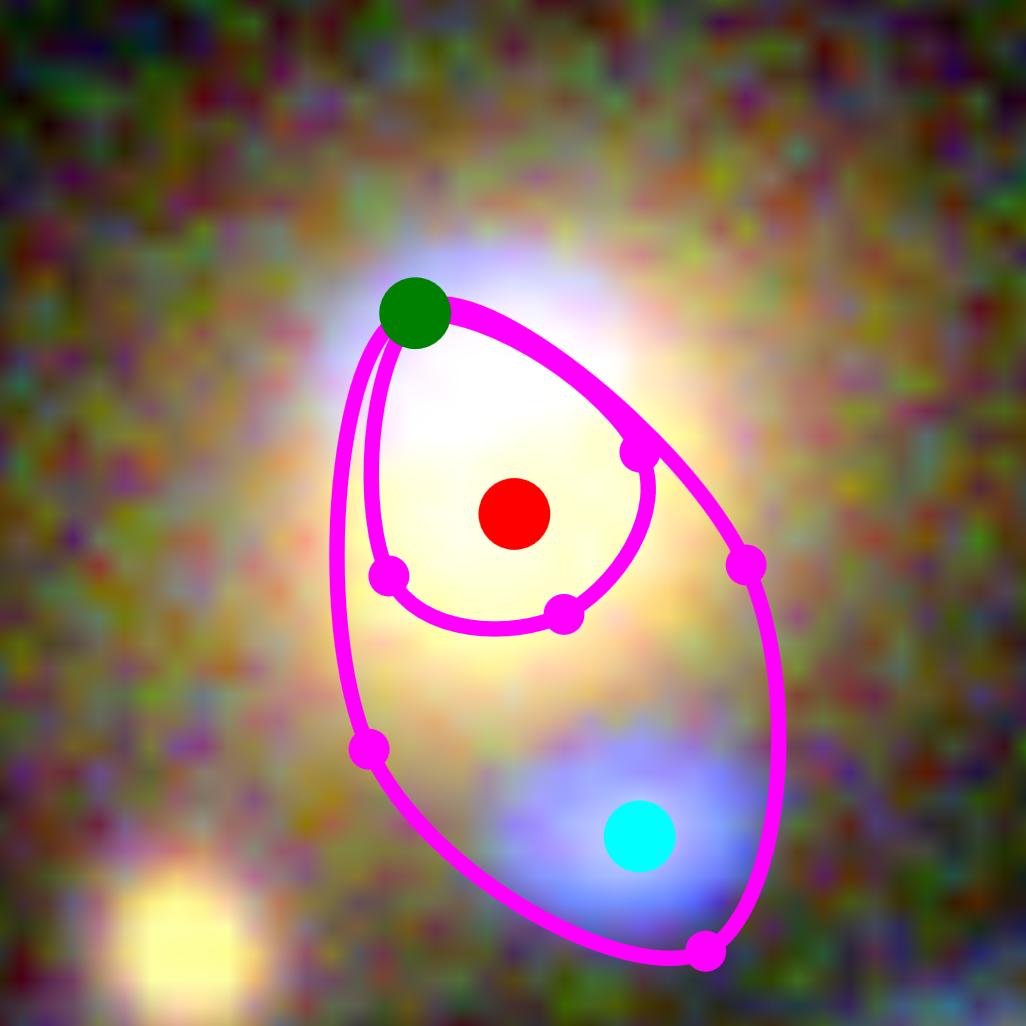
\includegraphics[width=\myplotswidth]{fig/006937_input}
  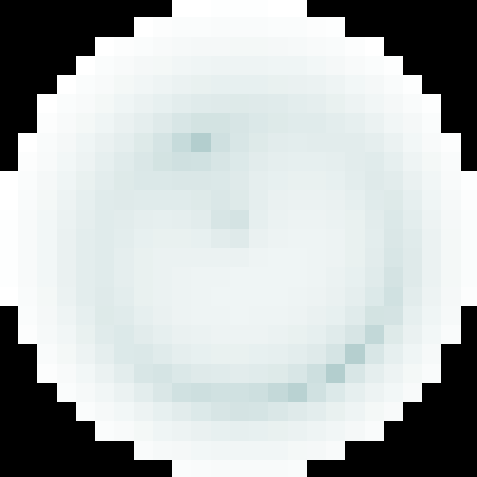
\includegraphics[width=\myplotswidth]{fig/006937_arr_time} \\
  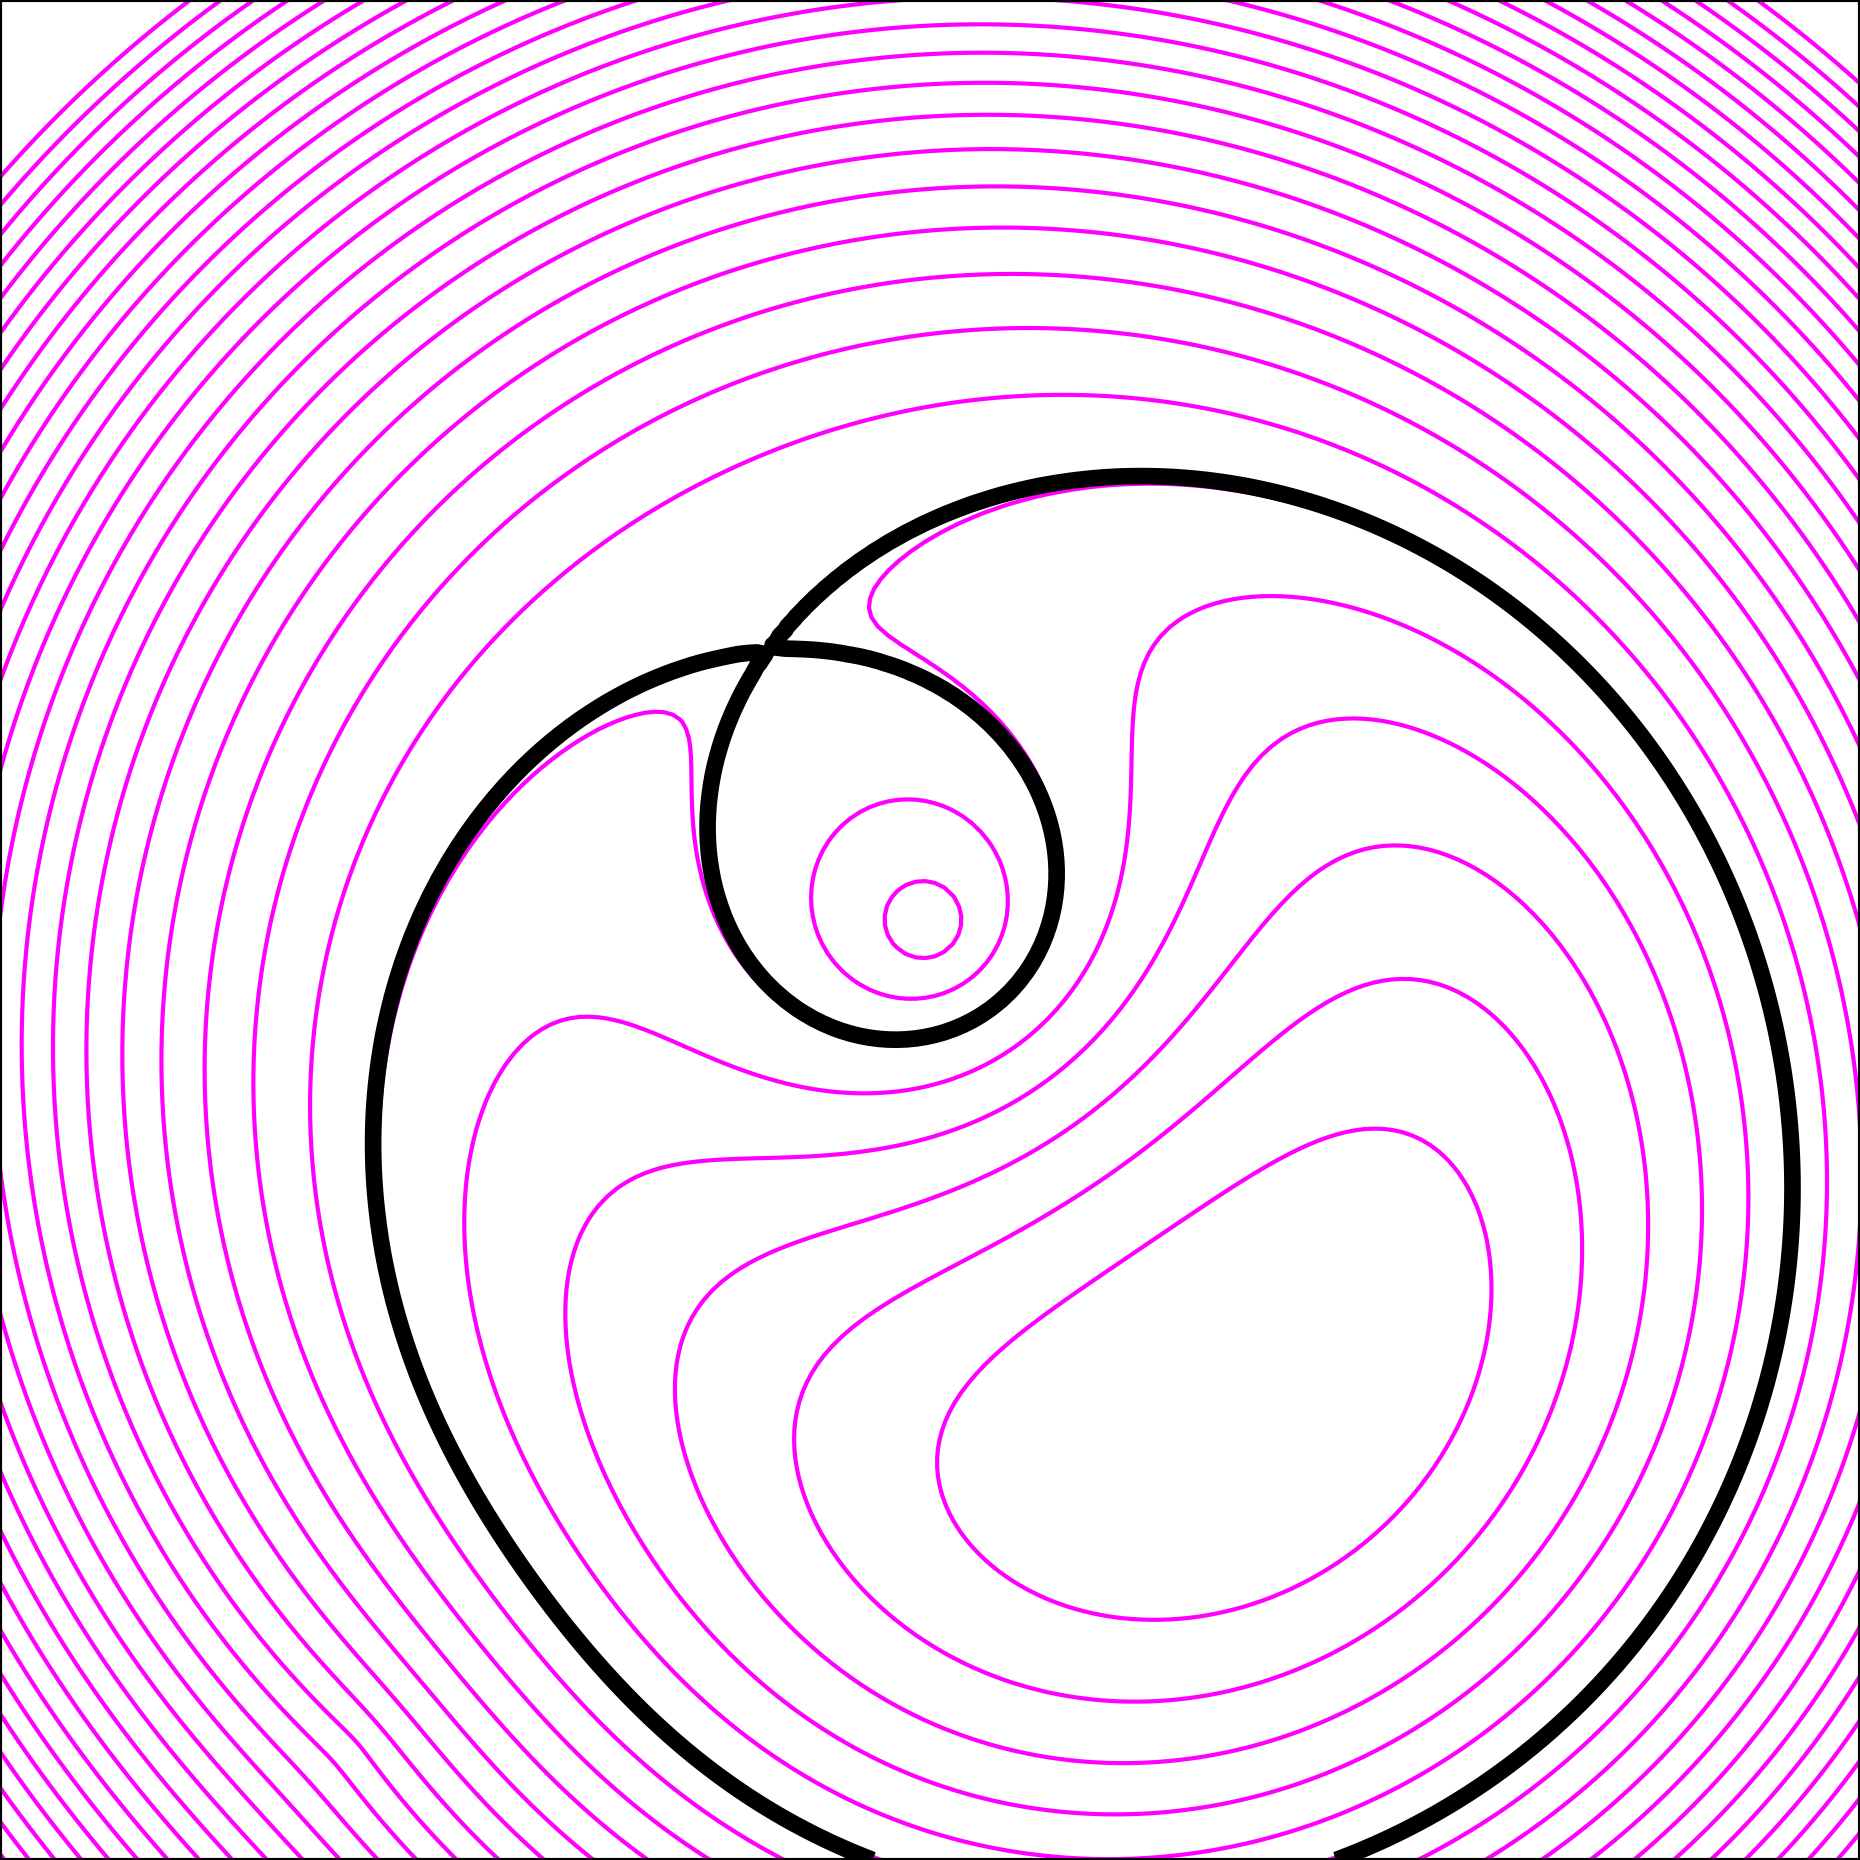
\includegraphics[width=\myplotswidth]{fig/ASW0000vqg_006937_arriv}
  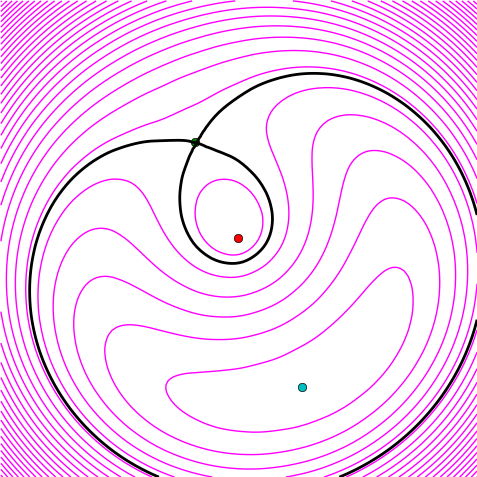
\includegraphics[width=\myplotswidth]{fig/006937_spaghetti} \\
  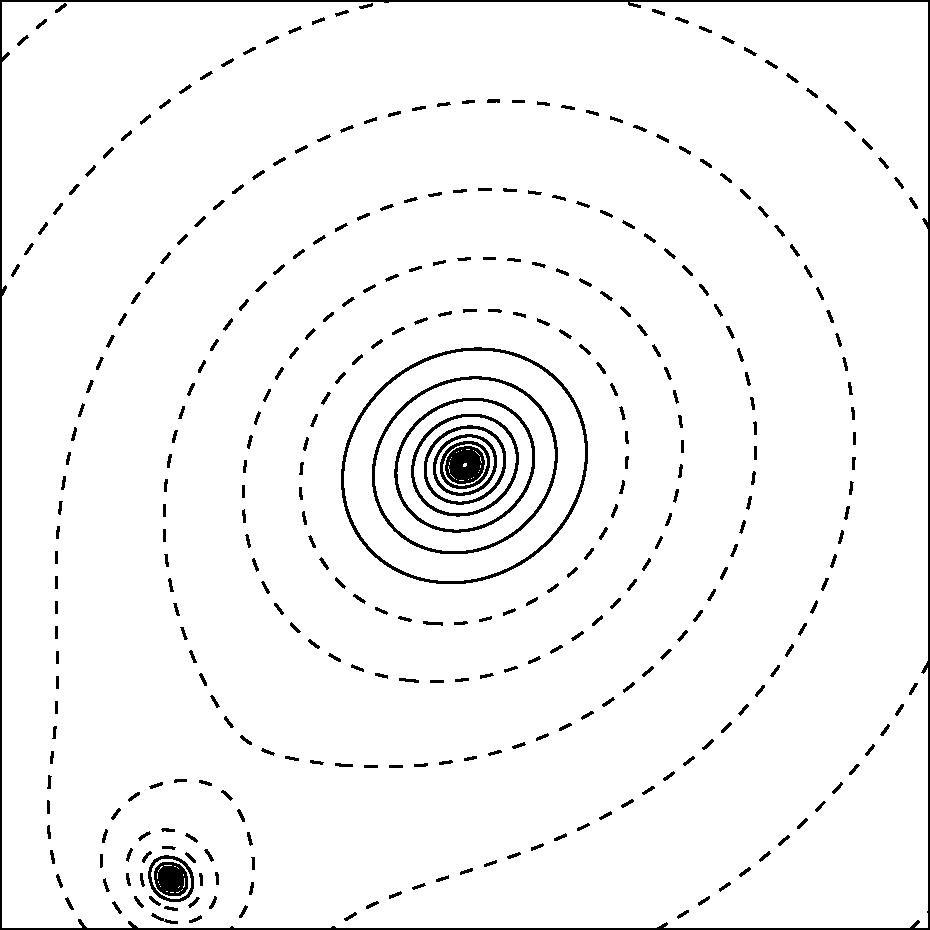
\includegraphics[width=\myplotswidth]{fig/ASW0000vqg_006937_kappa}
  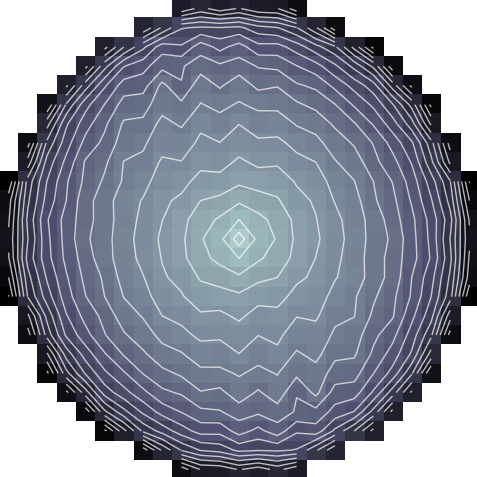
\includegraphics[width=\myplotswidth]{fig/006937_mass}

  \caption[result 6937 (ASW0000vqg)]{A sim with unrecovered
    substructure, resulting in a poor mass model. (See Section
    \ref{sec:example_models} for details.)}
  \label{fig:6937}
\end{figure}




\begin{figure}
  \centering

  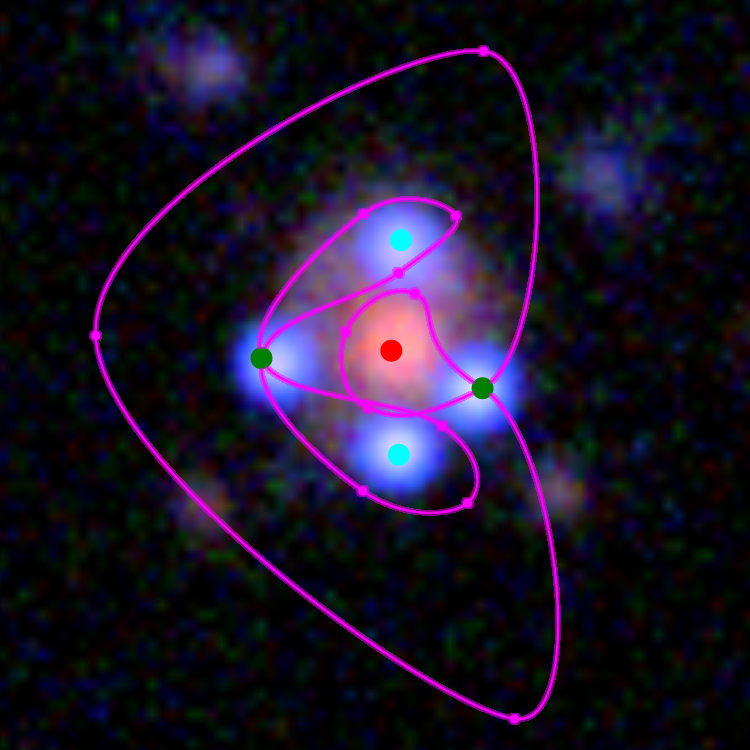
\includegraphics[width=\myplotswidth]{fig/007025_input}
  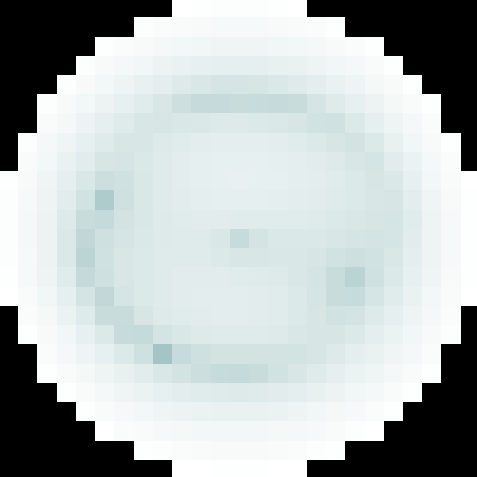
\includegraphics[width=\myplotswidth]{fig/007025_arr_time} \\
  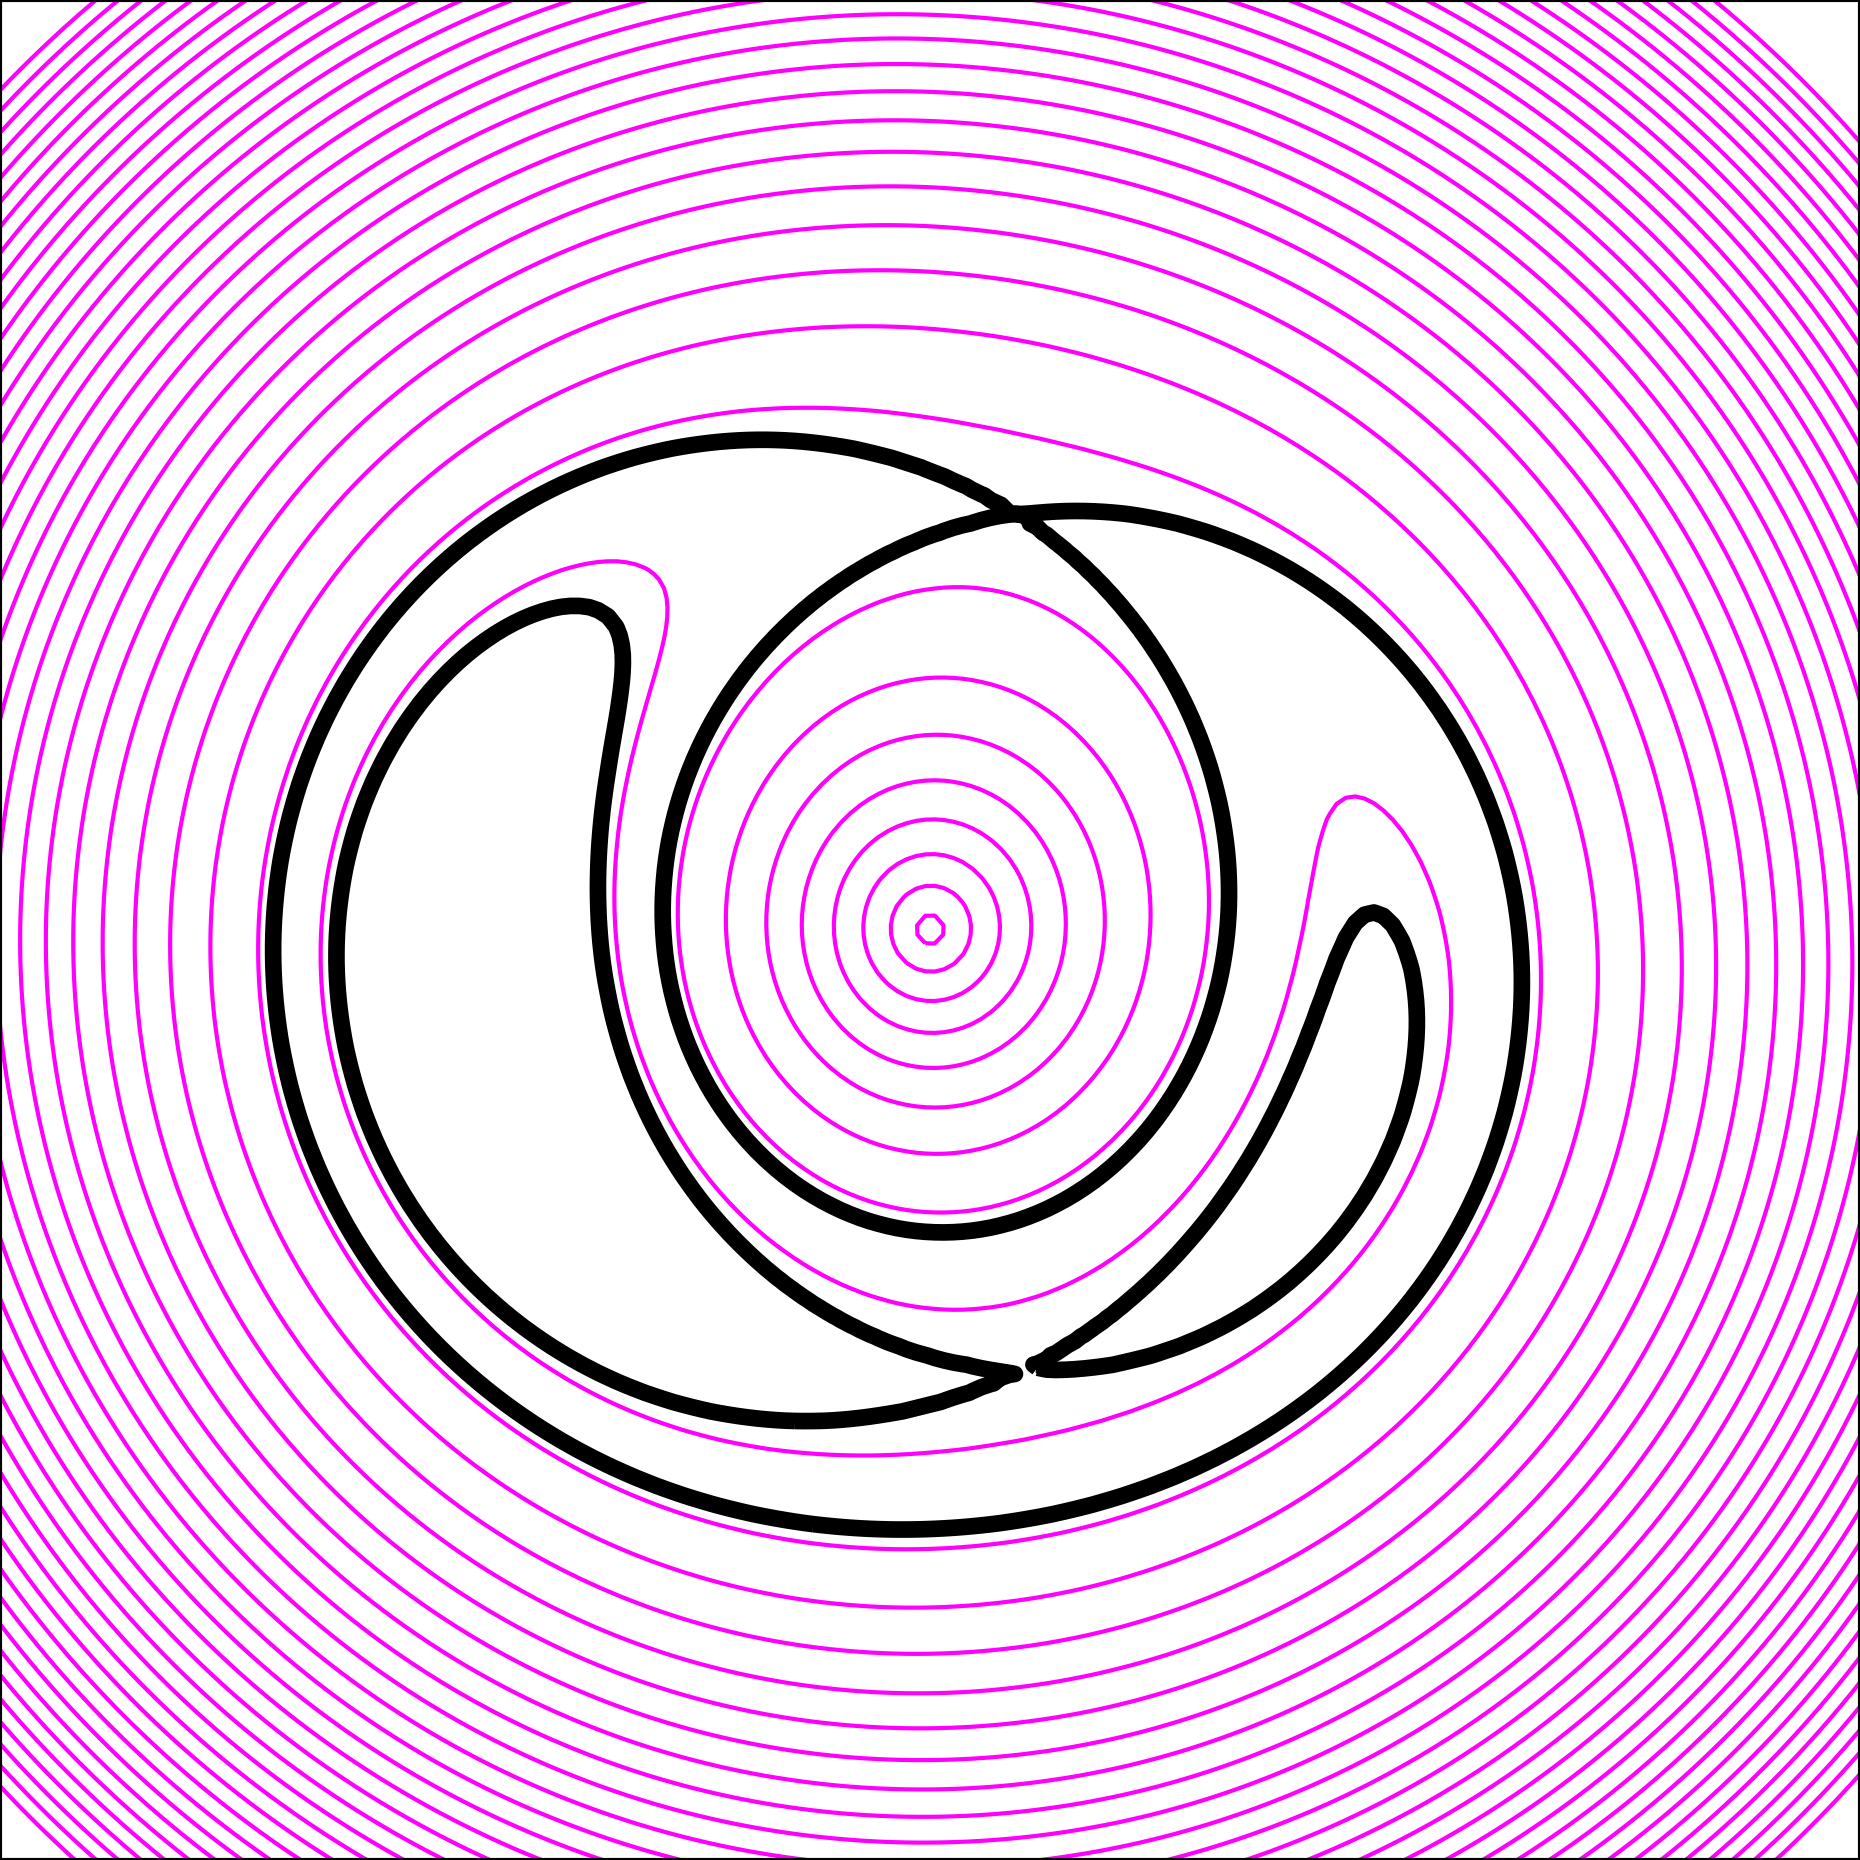
\includegraphics[width=\myplotswidth]{fig/ASW0000h2m_007025_arriv}
  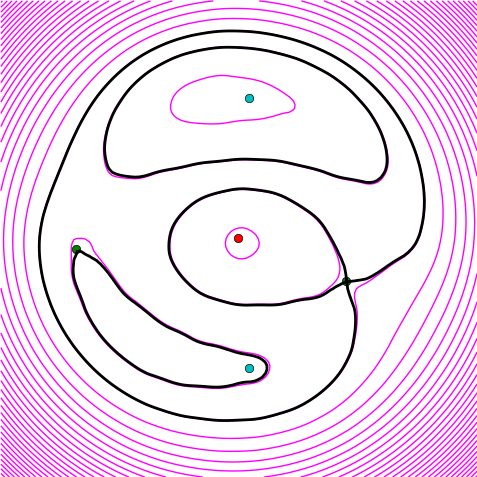
\includegraphics[width=\myplotswidth]{fig/007025_spaghetti} \\
  \includegraphics[width=\myplotswidth]{fig/ASW0000h2m_007025_kappa}
  \includegraphics[width=\myplotswidth]{fig/007025_mass}
  \caption[result 7025 (ASW0000h2m)]{A four-image system with image
    parities incorrectly identified.  The model is poor, but the
    estimated Einstein radius is not bad. (See Section
    \ref{sec:example_models} for details.)}
  \label{fig:7025}
\end{figure}

\begin{figure}
  \centering


  \includegraphics[width=\myplotswidth]{fig/007022_input}
  \includegraphics[width=\myplotswidth]{fig/007022_arr_time} \\
  \includegraphics[width=\myplotswidth]{fig/ASW0000h2m_007022_arriv}
  \includegraphics[width=\myplotswidth]{fig/007022_spaghetti} \\
  \includegraphics[width=\myplotswidth]{fig/ASW0000h2m_007022_kappa}
  \includegraphics[width=\myplotswidth]{fig/007022_mass}

  \caption[result 7022 (ASW0000h2m)]{The same system as in Figure
    \ref{fig:7025}, this time with image parities correctly
    identified. (See Section \ref{sec:example_models} for details.)}
  \label{fig:7022}
\end{figure}



\newpage

Figure \ref{fig:6941} shows a simple example.  The top two panels show
contours of convergence $\kappa(x,y)$, and of the arrival-time for a
point source at the brightest point of the sim
source.\footnote{Although the arrival-time contours represent an
  abstract quantity that is not directly observable, the contour map
  may actually resemble the appearance of the lensed arcs.  The
  resemblance is due to a serendipitous computer-graphical effect
  \citep{2001AJ....122..585S}.} The spatial scale is in pixels.  The
information in these two panels was, of course, kept secret during the
modeling challenge.  The panels in the middle row and at the lower
right are the results that \spl returns to the modeler, in order for
them to assess the model.  These derive from the mean of an ensemble
of 200 models generated by \spl.  The model mass distribution (left mid) is
returned as a contour map superimposed on an intensity map. A fairly
smooth mass distribution, as here, is a good sign.  An irregular or
checkboard pattern in the mass map usually indicates a bad model.  The
models arrival-time contours are shown in the right middle panel.
  The special contour passing through a
saddle point is shown in black: this is the model version of the
spaghetti sketch provided by the user.  Also provided is a synthetic
image of the lensed source in the bottom right panel.
  For this, \spl assumes a simple conical
source profile.  The user can change the contrast level on the image,
which (though it is not saved) amounts to adjusting the width of
the cone.  Finally, to the lower left of the figure, we have a
comparison of the input and recovered mass profiles.  The panel shows
a average $\kappa$ within a given radius, as a function of radius.
The red curve is the true value, and where it crosses unity (dotted
horizontal line) is the notional Einstein radius $\Theta_{\text{E, sim}}$.
  The two blue curves
are the minimal and maximal mean enclosed $\kappa$ from the internal
ensemble in \spl.  The region between the blue curves is shaded
between the radii of the innermost and the outermost images --- this
is the confidence region from the modeling.  As we see, the shaded
blue is slightly above the red curve. 
The Einstein Radius $\Theta_\text{E}$ of the model is estimated crossing the
mean enclosed $\kappa$ (not plotted) with unity.
  In summary: the identification
of minimum and saddle point is correct, but the estimated Einstein
radius is a little too high.

Figure \ref{fig:6975} shows a lens with substructure in the form of a
smaller secondary galaxy.  The galaxies in such group or cluster sims
were, in fact, based on galaxies visible in the images --- but the
modelers were not told in advance whether this was the case.  The
model does not include any substructure, but otherwise is not bad.
The minimum and saddle point are correct, and the Einstein radius is
only a little underestimated.

Figure \ref{fig:6937} shows a case where substructure leads to a
poor model.

Figure \ref{fig:6990} shows an example of an arc that has split into
three images.  This kind of configuration, with a counter-image close
to the lensing galaxy and a more distant arc/triplet on the other
side, generically arises from an elongated mass distribution when the
source is displaced along the elongated direction.

Figure \ref{fig:6915} shows another quad.  This kind of configuration
arises when the mass is elongated and the source is displaced at an
angle to the elongation.

Figure \ref{fig:6975} shows a fairly symmetric quad.  The minima and
saddle points are correctly identified, and the orientation of the
ellipticity of the mass distribution is correctly reproduced.  The
Einstein radius is somewhat overestimated.  Figure \ref{fig:7022}
shows another model of the same system.  In this one, the
identification of the minima and saddle points was incorrect, and mass
distribution comes out elongated East-West instead of North-South.
The mass distribution also appears somewhat jagged and the
saddle-point contours are not as clean as in the previous examples;
these are often indicators of a problem with the model.  The enclosed
mass is, however, none the worse --- the reason is probably that in a
relatively symmetrical image configuration, the Einstein radius is quite
well constrained by the images in a fairly model-independent way.

To conclude this set of examples, Figure \ref{fig:6919} shows another
type of quad.  Actually, in this case the brightest part of the source
is only doubly imaged, but the source extends into a region that
produces four images.  We can also see from the real arrival-time
surface that a point source is a double on the verge of splitting into
a quad.  The modeler interpreted the system as a quad.  The
appearance of the arcs, shown in the bottom panel of Figure
\ref{fig:input-spag}, looks like an arc and counter-image such as
discussed with Figure \ref{fig:6990} above.  But there is an important
difference: the long arc is closer to the galaxy, as if the arc and
counter-image have swapped roles.  This configuration arises if the
source displacement is perpendicular to the long axis of the lensing
mass.

